\chapter{Analyse de la distribution d'un marqueur de l'attention au sein d'une population d'enfants TDAH} \label{chapitre-4}

\section*{Introduction}
Il existe de nombreuses études sur les distributions de \gls{tbr} chez les enfants souffrant de \gls{tdah}
\citep{Arns2013, Clarke2001, Zhang2017}. Cela constitue par ailleurs la base historique de l'apparition du protocole de \gls{nfb} qui consiste à diminuer le \gls{tbr} 
comme intervention utilisée
pour traiter le \gls{tdah} chez les enfants \citep{Arnold2014, Deilami2016, Gevensleben2009, VanDongen2013}. Cependant, ce protocole ne serait 
peut-être pas adapté à tous les enfants souffrant de \gls{tdah} si 
l'on prend en compte la variété de phénotypes \gls{eegi} présents. En effet, il a été avancé qu'il existerait un groupe d'enfants \gls{tdah} présentant un \gls{tbr} élevé 
\citep{Zhang2017, Clarke2011}, ainsi ces enfants bénéficieraient peut-être davantage d'un protocole diminuant leur \gls{tbr} que les autres. 

Quelques études ont proposé de personnaliser le protocole d'entrainement par \gls{nfb} \citep{Bazanova2018, Escolano2014}, mais trop peu pour en déterminer
l'impact sur l'efficacité du \gls{nfb} par la \gls{saob} présenté dans le chapitre \ref{ch-saob}. L'analyse présentée dans cette partie n'a pas pour but d'évaluer directement l'efficacité de la 
personnalisation des protocoles de \gls{nfb}, mais d'en étudier la pertinence. Pour ce faire, la distribution des valeurs de \gls{tbr} chez les enfants \gls{tdah} est 
étudiée à l'aide de différentes méthodes de partitionnement (\textit{clustering} en anglais) pour déterminer des groupes d'enfants \gls{tdah} en se basant seulement sur les 
valeurs de \gls{tbr}. 
\newpage

\section{Population étudiée}

Les signaux \gls{eegi} utilisés dans cette analyse proviennent de trois bases de données différentes :
\begin{itemize}
\item NEWROFEED (NCT02778360, Mensia Technologies, France, ClinicalTrials.gov, \citet{Bioulac2019}),
\item \gls{cmi-mipdb} \citep{Langer2017, Langer2017b}, les signaux \gls{eegi} sont accessibles en \href{http://fcon_1000.projects.nitrc.org/indi/cmi_eeg/eeg.html}{ligne},
\item \gls{cmi-hbn} \citep{Alexander2017, Alexander2017b}, pour laquelle les signaux sont également disponibles en 
\href{http://fcon_1000.projects.nitrc.org/indi/cmi_healthy_brain_network/sharing_neuro.html}{ligne}.
\end{itemize}
Pour chacune de ces bases de données, un consentement éclairé écrit a été obtenu de tous les participants ou de leurs responsables légaux. Tous les enregistrements
ont été effectués dans un environnement contrôlé avec les yeux ouverts (\gls{eo} en anglais) et au repos (c'est à dire que le sujet n'effectue aucune tâche) 
pendant une minute sous la supervision d'un spécialiste. 

La description de l'ensemble des données est disponible dans la Table~\ref{Table:tbr_datasets_description}. Au total, les enregsitrements \gls{eegi} de 
$n = 363$ sujets diagnostiqués \gls{tdah} sont analysés.

\begin{table}[h!]
  \centering
  \caption[Informations sur les données utilisées.]{Informations sur les données utilisées. Les critères d'inclusion pour chaque base de données sont listés, ainsi que le nombre de sujets satisfaisant
	chaque critère entre parenthèses. Le nombre total de sujets inclus par base de données est précisé à la dernière ligne.}
  \fontsize{9}{11}\selectfont
\begin{tabular}{ ccccc }
\toprule
Base de données & NEWROFEED & CMI-MIPDB & \multicolumn{2}{ c }{CMI-HBN} \\
\midrule
\shortstack{ Description \\ de la population } & \shortstack{ - 7-13 ans \\ - Diagnostiqué \gls{tdah} \\ - Enregistré avec \\ l'appareil
                                               \\ Mensia Koala\textregistered : \\ 8 électrodes \\ du système 10-20 } 
																							 & \shortstack{ - 6-44 ans \\ - Avec et sans \\ diagnostic \\ - Enregistré avec \\ le système
                                               \gls{eeg} \\ Geodesic Hydrocel : \\ 128 électrodes } 
																							 & \multicolumn{2}{ c }{ \shortstack{ - 5-21 ans \\ - Avec et sans \\ diagnostic \\ - Enregistré avec \\ le système
                                               \gls{eeg} \\ Geodesic Hydrocel : \\ 128 électrodes } }
																							\\
\midrule
Nombre de sujets & \shortstack{ 122 (données disponibles \\ au 09/2017 pour les \\ analyses de contrôle \\ de la qualité avant \\ la fin de l'étude \\ en 12/2017) } 
                 & 126 
								 & \multicolumn{2}{ c }{ 881 }
								\\
\midrule
\shortstack{ Critères d'inclusion \\ additionnels} & \shortstack{ 1. Age/diagnostic \\ précisés (122) \\ 2. \textbf{Diagnostic} \\ \textbf{ \gls{tdah} } (122) \\ 3. \gls{eeg} d'une \\ min \gls{eo} 
                 au repos \\ disponible et \\ possible à \\ analyser (122) } 
                 & \shortstack{ 1. Age/diagnostic \\ précisés (126) \\ 2. \textbf{Diagnostic :} \\ \textbf{ \gls{tdah} } (12) \\ 3. \gls{eeg} d'une \\ min \gls{eo} 
                 au repos \\ disponible et \\ possible à \\ analyser (10) } 
								 & \shortstack{ 1. Age/diagnostic \\ précisés (447) \\ 2. \textbf{Diagnostic :} \\ \textbf{ \gls{tdah} } (237) \\ 3. \gls{eeg} d'une \\ min \gls{eo} 
                 au repos \\ disponible et \\ possible à \\ analyser (231) } 
								 & \shortstack{ 1. Age/diagnostic \\ précisés (447) \\ 2. \textbf{Diagnostic :} \\ \textbf{ Aucun }  (76) \\ 3. \gls{eeg} d'une \\ min \gls{eo}  
                 au repos \\disponible et \\ possible à \\ analyser (74) } 
								\\
\midrule
\shortstack{ Nombre de \\ sujets inclus} & 122 & 10 & 231 & 74 \\
\bottomrule
\end{tabular}
  \label{Table:tbr_datasets_description}
\end{table}

Les trois bases de données diffèrent les unes des autres, notamment celle de NEWROFEED dont les \gls{eeg} ont été enregistrés avec moins d'électrodes 
que ceux issus des bases de données du \gls{cmi}. Ainsi, une fois que chaque base a été décrite, les étapes
mises en place pour homogénéiser l'ensemble des données sont explicitées.

\subsection{Données NEWROFEED}

Une partie des données utilisées dans cette analyse provient de l'étude NEWROFEED (NCT02778360, Mensia Technologies, France, ClinicalTrials.gov, \citet{Bioulac2019})
qui avait pour but d'évaluer si l'efficacité du \gls{nfb} à la maison était non-inférieure à celle du \gls{mph} sur une population d'enfants souffrant du \gls{tdah}.
Au moment où le travail décrit dans ce chapitre a été mené, NEWROFEED était en cours, donc 
seulement une partie des données était disponible. Ainsi, 122 enregistrements \gls{eegi} d'enfants diagnostiqués \gls{tdah} d'après les critères du DSM-IV \citep{DSM-4} 
ont été analysés. L'\gls{eeg} a été enregistré avec l'appareil Mensia Koala équipé de 8 électrodes \gls{agcl} individuellement blindées, positionnées sur le scalp en accord avec 
le système international 10-20 : Fpz, F3, Fz, F4, C3, Cz, C4, Pz. La fréquence d'échantillonnage était de 512Hz. Les impédances devaient être
inférieures à $40\text{k}\Omega$ et le niveau de contamination électromagnétique devait rester inférieur à 1/3 de l'énergie totale du signal. 

Pour participer à l'étude NEWROFEED, les sujets devaient remplir les critères suivants :
\begin{enumerate}
\item être des enfants ou adolescents (fille ou garçon) entre 7 et 13 ans,
\item avoir un diagnostic \gls{tdah} positif avec Kiddie-SADS \citep{Kaufman1997},
\item avoir un score sur l'ADHD Rating Scale IV supérieur à 6 pour l'inattention, avec ou sans hyperactivité \citep{Pappas2006}.
\end{enumerate}

De plus, les enfants correspondant à un de ces critères ont été exclus :
\begin{itemize}
\item être \gls{tdah} avec le sous-type hyperactif/impulsif mais sans la composante inattention,
\item avoir un trouble psychiatrique sévère et/ou incontrôlable autre que le \gls{tdah} diagnostiqué avec Kiddie-SADS tel que par 
exemple l'autisme ou la schizophrénie,
\item avoir un trouble comorbide nécessitant des médicaments psychoactifs autres que ceux prescrits pour le \gls{tdah},
\item avoir un \gls{qi} < 80 d'après les trois sous-tests du \gls{wasi} ou du \gls{wisc} \citep{Wechsler1999}.
\end{itemize}

Seule la première évaluation de l'\gls{eeg} enregistrée pour chaque patient avant le début du traitement par \gls{nfb} ou du traitement par \gls{mph} est utilisée pour cette analyse. 
L'étude NEWROFEED a été menée dans 12 centres cliniques dans 5 pays européens (France, Espagne, Allemagne, Belgique et Suisse).

\subsection{Données CMI-MIPDB}
Au moment de l'analyse, l'intégralité de la base \gls{cmi-mipdb} compte 126 participants à la fois avec et sans diagnostic clinique \citep{Langer2017, Langer2017b}.
Les participants ont été recrutés au Child Mind Medical Practice et dans la région de la ville de New-York. Chaque sujet a été questionné pendant 10 minutes
au téléphone ou en personne par un chercheur expérimenté pour évaluer son éligibilité grâce à :
\begin{itemize}
\item l'historique des troubles psychiatriques, incluant les traitements en cours et précédents,
\item l'historique des troubles neurologiques et/ou épilepsie.
\end{itemize}

L'enregistrement de l'\gls{eeg} est prévu si aucune contre-indication n'est trouvée. 

De tous les patients présents dans la base \gls{cmi-mipdb}, seulement ceux satisfaisant aux critères suivants ont été inclus dans l'analyse présentée dans ce chapitre :
\begin{enumerate}
\item être diagnostiqué \gls{tdah} d'après les critères du DSM-IV \citep{DSM-4},
\item posséder un \gls{eeg} au repos disponible au format brut (c'est à dire sans pré-traitement),
\item avoir son âge précisé.
\end{enumerate}

L'\gls{eeg} a été enregistré avec un système \gls{eegi} Geodesic Hydrocel \gls{egi} à une fréquence d'échantillonnage de 500Hz et filtré entre 0.1 et 100Hz. 
L'électrode de référence est Cz, localisée au vertex de la tête. Le tour de tête de chaque participant est mesuré pour que le bonnet utilisé lors de l'enregistrement 
soit à la bonne taille. L'impédance des électrodes est gardée inférieure à $40\text{k}\Omega$ : elle est vérifiée toutes les 30 minutes ainsi qu'avant chaque enregistrement.

\subsection{Données CMI-HBN}
La base de données \gls{cmi-hbn} est composée de 881 sujets, avec ou sans diagnostic \citep{Alexander2017, Alexander2017b}. Les familles reçoivent 150\$ pour leur participation 
et les sujets bénéficient des rapports de consultation et des avis sur leurs sessions d'\gls{eegie}.

Seuls les sujets remplissant les critères suivants ont été inclus dans notre analyse :
\begin{enumerate}
\item être diagnostiqué \gls{tdah} selon le KSADS-COMP \citep{Kaufman1997},
\item posséder un \gls{eeg} au repos disponible au format brut (c'est à dire sans pré-traitement),
\item avoir son âge précisé.
\end{enumerate}

Des 881 sujets disponibles, 231 (âgés entre 5 et 21 ans) satisfont ces critères et sont inclus dans notre analyse.

La base de données \gls{cmi-hbn} contient également des sujets sains qui vont être utilisés en tant qu'\textit{a priori} (\textit{priors} en anglais) pour le
modèle bayésien décrit en \ref{clustering}. Pour être inclus dans cette analyse en tant que \textit{priors}, les sujets ne doivent avoir aucun diagnostic 
et doivent remplir les critères 2. et 3. cités précédemment. Au final, 74 sujets entre 5 et 21 ans sont sélectionnés. 

\subsection{Pré-traitement et homogénéisation des bases de données} \label{pré-traitement TBR}
Les \gls{eeg} des différentes bases de données sont pré-traités de façon à être comparables, notamment au niveau du placement des électrodes.
En ce qui concerne le traitement des artefacts et l'extraction du \gls{tbr}, les étapes sont les mêmes quelle que soit la base de données. 
Les pré-traitements ainsi que les analyses des signaux \gls{eegi} qui suivent sont effectués à l'aide du logiciel NeuroRT (v3, Mensia Technologies, 
Paris, France).

\subsubsection{Base de données NEWROFEED}
Le seul pré-traitement que nécessitent les signaux de la base de données NEWROFEED est un filtrage temporel : 
\begin{itemize}
\item un filtre Butterworth passe-haut d'ordre 1 à 0.5Hz afin d'enlever la composante continue (\textit{DC component} en anglais),
\item un filtre Butterworth coupe-bande d'ordre 3 de 47 à 53Hz afin d'enlever l'artefact causé par les lignes électriques.
\end{itemize}

\subsubsection{Bases de données \gls{cmi}} \label{treatment_cmi_databases}

Le pré-traitement des bases de données \gls{cmi-mipdb} et \gls{cmi-hbn} demande plus d'étapes : filtrage temporel, suppression et 
interpolation des canaux bruités et/ou déconnectés, et une interpolation spatiale afin de passer d'un espace à 128 électrodes \gls{egi}
à l'espace de 8 électrodes placées selon le système 10-20, utilisé dans la base de données NEWROFEED.

Tout d'abord, les \gls{eeg} obtenus au repos sont séparés en deux fichiers : l'un pour les enregistrements les yeux fermés, 
l'autre pour les enregistrements \gls{eo}, seul ce dernier va être analysé. Ensuite, les mêmes filtres temporels vont être appliqués
que pour les données NEWROFEED, à l'exception du filtre coupe bande dont les bornes sont modifiées pour intercepter les artefacts 
causés par les lignes électriques américaines (57-63Hz).

Dans le cas d'enregistrements d'\gls{eegi} avec une haute résolution spatiale comme ici avec les données \gls{cmi}, 
il est courant qu'au moins un canal se déconnecte ponctuellement causant aussi bien des artefacts de large amplitude que des signaux plats \citep{Barlow1986, Oregan2013}. 
Une strategie est ici mise en place pour détecter de façon fiable ces électrodes déconnectées puis pour les interpoler : la variance de chaque canal 
\gls{eegi} est calculée sur une fenêtre glissante de 10 secondes puis est ensuite convertie en deux $Z$-scores grâce à :
\begin{enumerate}
\item la distribution instantanée des variances pour les 127 autres canaux ($Z$-score spatial),
\item la distribution cumulative des variances pour le canal d'intérêt ($Z$-score temporel).
\end{enumerate}
Si le $Z$-score temporel n'est pas compris entre -5 et 5, le signal est détecté comme étant un artefact et est interpolé à partir des canaux voisins.
Si le $Z$-score spatial n'est pas compris entre -2 et 2, soit le signal a une trop grande variance (autrement dit il est bruité), soit une trop faible
variance (autrement dit l'électrode doit être déconnectée et n'enregistre rien) : dans les deux cas il est interpolé. Ces valeurs ont été choisies
empiriquement en se basant sur la distribution des variances mais n'ont pas été validées de manière plus précise.  

Les données sont re-référéncées sur l'électrode de la mastoïde gauche (électrode 57 de l'\gls{egi}-128) pour correspondre au référencement de la base
de données NEWROFEED. Les signaux \gls{eegi} des 128 électrodes de l'espace \gls{egi} sont ensuite spatialement reconstruits dans l'espace à 8 électrodes 
dans le système international 10-20 en projetant les coordonnées sur une sphère unitaire \citep{Perrin1989}.


\section{Theta-Beta ratio : un marqueur de l'attention}

Le \gls{tbr} est un neuromarqueur couramment utilisé en \gls{nfb} appliqué aux enfants \gls{tdah} \citep{Arns2013}. L'utilisation fréquente de ce protocole est notamment due
à \citet{Lubar1991} qui, en se basant sur la littérature existante, avance que la valeur du \gls{tbr} permettrait de différencier un enfant \gls{tdah} d'un enfant sain.  

Le \gls{tbr} est d'abord défini, puis les étapes pour l'extraire des
signaux \gls{eegi} à notre disposition sont décrites. Ces \gls{tbr} sont ensuite partitionnés à l'aide de trois méthodes dont le principe est expliqué dans cette partie. 
Enfin, la méthode pour identifier le seuil optimal séparant les classes obtenues est détaillée.

\subsection{Définition du Theta-Beta ratio}
De précédentes études ont montré que les enfants souffrant de \gls{tdah} présentent une augmentation
de la puissance des ondes lentes et/ou une diminution de la puissance des ondes rapides
comparés aux enfants sains. Ces différences d'activité de ces 
ondes peuvent être quantifiées en calculant le ratio de la puissance dans la bande theta et de la puissance dans la bande beta : le 
\gls{tbr} \citep{Arns2013}, qui serait élevé chez les enfants souffrant du \gls{tdah} \citep{Lubar1991, Monastra1999, Barry2009, Snyder2006}. 

Au vu de cette observation, de nombreuses études ont été menées pour analyser la pertinence d'utiliser le \gls{tbr} comme biomarqueur pour 
diagnostiquer le \gls{tdah} comme suggéré par \citet{Lubar1991}. 
Par exemple, \citet{Monastra1999} ont mené une étude multicentrique sur 482 participants pour déterminer s'ils étaient ou non \gls{tdah} en se basant sur leur \gls{tbr} : 
ils ont obtenu une spécificité (capacité du test à ne détecter que les malades) de 98\% et une sensibilité (capacité du test à détecter tous les malades) de 86\%. 

Ainsi, un \gls{tbr} élevé pourrait aider à confirmer les diagnostics du \gls{tdah} : la \gls{fda} a d'ailleurs approuvé en 2013 le recours à la valeur du 
\gls{tbr} dans ce but \citep{NebaHealth, FDA, Saad2018, Barry2009}. Cependant, les études récentes ont échoué à répliquer les résultats
montrant une différence entre les valeurs de \gls{tbr} des patients \gls{tdah} et celles des enfants sains, remettant en question son utilisation comme outil 
diagnostic \citep{Zhang2017, Arns2013, Clarke2001, VanDoren2017, Lenartowicz2014}. A la place, les chercheurs suggèrent de se baser sur le \gls{tbr} à des fins prognostiques : l'\gls{eeg} 
serait analysé dans le but de prédire les différences entre les individus atteints du \gls{tdah} plutôt que dans celui d'identifier 
des caractéristiques du \gls{tdah} \citep{Arns2013, Zhang2017}. 

Cette utilisation prognostique du \gls{tbr} est notamment justifiée par \citet{Clarke2011} qui estiment qu'environ 35\% d'enfants \gls{tdah} présentent un \gls{tbr} élevé, ainsi que 
par des études qui montrent que la prise de stimulants chez les patients \gls{tdah} avec un \gls{tbr} élevé serait plus efficace \citep{Arns2012med, Clarke2002}. 
Ainsi, l'existence d'un groupe d'enfants \gls{tdah} au \gls{tbr} élevé pourrait être utilisée pour identifier de meilleurs répondeurs à une intervention donnée, comme le \gls{nfb}. 

La diminution du \gls{tbr} est l'objectif du protocole le plus couramment utilisé en \gls{nfb} appliqué aux enfants \gls{tdah} \citep{Arns2014}. 
On peut supposer que l'efficacité de ce traitement pourrait être augmentée en affectant chaque patient à l'entraînement qui correspond le mieux à son phénotype \gls{eegi}. 
Par exemple, il serait peut-être plus pertinent que les sujets présentant un haut \gls{tbr} suivent un protocole de \gls{nfb} où il est demandé de 
diminuer le \gls{tbr}. Cette répartition a été proposée lors de l'essai clinique NEWROFEED, pour lequel un seuil de répartition a dû être choisi pour allouer les sujets 
selon leur valeur de \gls{tbr} à l'un des protocoles de \gls{nfb} disponibles (diminution du \gls{tbr} ou augmentation du \gls{smr}). 
Un autre essai clinique randomisé et en double aveugle proposé par \citet{Kerson2013} prévoyait d'inclure des enfants entre 7 et 10 ans présentant un \gls{tbr} supérieur à 5 mais cette valeur a 
été modifiée et fixée à 4.5 (NCT02251743, Arnold, Ohio State University, ClinicalTrials.gov), valeur également
utilisée dans NEWROFEED. Choisir correctement la valeur de seuil est crucial car cette valeur détermine quel protocole de \gls{nfb} le patient va suivre. 

Le caractère arbitraire des valeurs de seuil basées sur le \gls{tbr} appelle à une validation précise de l'existence d'un 
sous-groupe de patients \gls{tdah} présentant un \gls{tbr} élevé et du seuil à partir duquel les valeurs de \gls{tbr} sont considérées comme élevées.  
 
\subsection{Extraction du Theta-Beta ratio} \label{extraction_tbr}
L'extraction du \gls{tbr} des \gls{eeg} obtenus après les pré-traitements présentés en \ref{pré-traitement TBR} comprend plusieurs étapes :
\begin{enumerate}
\item le rejet des artefacts en utilisant la géométrie Riemannienne,
\item l'extraction de l'\gls{iapf},
\item le calcul du \gls{tbr}.
\end{enumerate}

\subsubsection{Rejet des artefacts}
Tout d'abord, les données artefactées sont exclues en utilisant le géométrie Riemanniene \citep{Barachant2013, Barthelemy2019}. 

Le principe de cette méthode consiste à calculer la matrice de covariance de chaque segment d'\gls{eeg} : les époques dont la matrice de covariance se trouve à l'extérieur d'une région
d'acceptabilité, appelée patate, définie par un $Z$-score sont considérées artefactées et donc rejetées. Cette région d'acceptabilité est définie par une référence d'\gls{eeg} propre.

Afin d'augmenter la sensibilité et la spécifité de cette méthode de rejet, plusieurs petites patates définies sur certains canaux peuvent travailler en parallèle \citep{Barthelemy2019}, 
cette méthode a été appliquée ici.
Les données \gls{eegi} sont segmentées (durée de 2 secondes avec un chevauchement toutes les 0.125s) et sont analysées simultanément par six patates. Chaque patate a pour but de détecter 
un type d'artefact, les canaux de chaque patate ainsi que le filtrage du signal \gls{eegi} sont donc choisis de façon à pouvoir le repérer. 
Les sous-ensembles de canaux choisis ici et les bandes de fréquence \gls{eegi} analysées sont les suivants :
\begin{itemize}
\item Fpz, F3, F4, C3 et C4 pour détecter les artefacts musculaires. Ces artefacts affectant les hautes fréquences, le signal a été préalablement filtré entre 55 et 95Hz,
\item quatre groupes de deux électrodes (Fpz et Fz, F3 et F4, C3 et C4, Cz et Pz) pour détecter les déconnections temporaires d'électrodes. Le signal a été préalablement filtré entre 1 et 20Hz, 
\item l'ensemble des canaux (Fpz, Fz, F3, F4, C3, C4, Cz et Pz) pour détecter les artefacts généraux. Le signal a été filtré de façon à exclure la bande de fréquences entre 4 et 31Hz, qui correspond
aux ondes \gls{eegi} d'intérêt.
\end{itemize}
Pour chaque patate un $Z$-score est calculé, ceux-ci sont ensuite combinés pour aboutir à une seule $p$-value : un segment d'\gls{eeg} est considéré comme propre si cette $p$-value est 
plus grande qu'un seuil obtenu grâce à une référence d'\gls{eeg} propres. 

\subsubsection{Extraction de l'\gls{iapf}} \label{extraction_iapf}
Ensuite, l'\gls{iapf}, définie en \ref{principe_nfb}, est calculée en déterminant la fréquence à laquelle le pic de puissance est observé dans la bande alpha prise entre 7 et 13Hz.
Cette bande de fréquence est extraite de l'\gls{eeg} enregistré à l'électrode Pz au repos et les yeux ouverts. 
Si aucun pic n'est détecté, l'\gls{iapf} est obtenue grâce à l'estimation de Klimesch basée sur l'âge du sujet \citep{Klimesch1999}. 

L'\gls{iapf} permet de définir des bandes de fréquence personnalisées pour chaque sujet qui ont été choisies 
par le comité scientifique de NEWROFEED : theta = [\gls{iapf} - 5Hz ; \gls{iapf} - 1Hz] et beta = [\gls{iapf} + 3Hz ; \gls{iapf} + 12Hz].
Cette étape a pour but d'adapter précisément l'entrainement aux spécificités neurodéveloppementales liées à l'âge de l'enfant \citep{Aurlien2004}. En effet, dans le cas des enfants, 
il serait possible de considérer 
des basses fréquences de la bande alpha comme appartenant à la bande theta, ce qui fausserait l'entrainement par \gls{nfb} car la modulation de mauvaises fréquences 
serait récompensée. Cette méthode mène évidemment à des résultats différents d'avec des bandes de fréquence aux bornes fixes \citep{Arns2008, Vollebregt2015} et a été 
l'objet de plusieurs études \citep{Kaiser2001, Bazanova2006, Vollebregt2015} dont les résultats montrent que cette personnalisation pourrait améliorer l'efficacité du protocole
\gls{tbr} pour le traitement du \gls{tdah}.

\subsubsection{Calcul du \gls{tbr}} \label{tbr_computation}
La dernière étape consiste à obtenir le \gls{tbr}, dont la méthode de calcul diffère selon les études.

En effet, la façon dont est calculé le \gls{tbr} est très variable dans la littérature, ce qui conduit à des valeurs variant entre 2 et 8 pour les sujets contrôles \citep{Arns2012,
Schutte2017}. La largeur de cet intervalle s'explique en partie par les diverses définitions du \gls{tbr} : le \gls{tbr} peut faire référence au ratio
des puissances ($\mu$V$^2$), des densités de puissance ($\mu$V$^2$/Hz), des tensions ($\mu$V) ou des densités de tensions ($\mu$V/Hz).  

Par ailleurs, comme souligné en \ref{extraction_iapf}, la définition des bandes de fréquence pour calculer le \gls{tbr} peut aussi varier : par exemple, le \gls{tbr} peut être obtenu à partir
de bandes de fréquence standards ou personnalisées grâce à l'\gls{iapf} du sujet. 

Dans notre cas le \gls{tbr} est défini comme le ratio de la puissance dans la bande de fréquence theta et de la bande de fréquence beta obtenues 
grâce à l'\gls{iapf}. Une moyenne mobile de la puissance du signal $\bar{P}$ est estimée par la méthode de Welch \citep{Welch1967} sur 32 segments, de 2 secondes chacun, avec un 
chevauchement toutes les 1/16 de seconde :
\begin{equation}
\label{eq:tbr_power_computation}
P_{c,b} = \norm{ x_{c,b} }_{F}^2,
\end{equation}
\begin{equation}
\label{eq:tbr_average_power_computation}
\bar{P}_{c,b} = \frac{1}{I} \sum_{i=1}^{I} (P_{c,b})_{i},
\end{equation}
où $x_{c,b}$ correspond à un segment du signal \gls{eegi} sur le canal $c$ après un filtre passe-bande sur la fréquence $b$, $\norm{.}_{F}$ est la norme de Frobenius et $I$ 
le nombre de segments. La puissance dans les bandes theta ($\theta$) et beta ($\beta$) est calculée avec les équations Eq.~(\ref{eq:tbr_power_computation}) et Eq.~(\ref{eq:tbr_average_power_computation}),
puis ces deux puissances sont divisées entre elles :

\begin{equation}
\label{eq:tbr_tbr_computation}
\text{TBR} = \frac{\bar{P}_{c,\theta}}{\bar{P}_{c,\beta}},
\end{equation}
conduisant à un ratio instantané de valeurs de puissances qui représente une implémentation en temps réel du \gls{tbr}.

La distribution de l'ensemble des $\bar{P}_{c,b}$ n'étant pas normale, la médiane obtenue à Fz et Cz est utilisée pour représenter le \gls{tbr} sur l'ensemble 
de l'enregistrement, puis le maximum sur ces deux électrodes est retenu.

Enfin, cette valeur de \gls{tbr} doit être normalisée pour les analyses de partionnement qui vont suivre. En effet, deux des méthodes utilisées pour modéliser la distribution des \gls{tbr},
le \glsfirst{bgmm} et le \gls{gmm} détaillées par la suite, supposent que la distribution des \gls{tbr} est normale. 
En effet, un \gls{bgmm} appliqué à une distribution non normale identifierait de faux groupes (\textit{clusters} en anglais) pour ajuster les données. 
Ainsi, pour être certain que l'hypothèse de normalité est valide, la distribution des \gls{tbr} de patients sains (provenant de la base de données \gls{cmi-hbn})
est analysée avec deux techniques de normalisation différentes : la \textit{log normalization} et la \textit{square-root-normalization}.

Les distributions de \gls{tbr} non-normalisés, log-normalisés et \textit{square-root} normalisés (les \gls{srntbr}) sont visuellement analysées à l'aide 
d'histogrammes, puis des tracés de probabilités (\textit{probability plots} en anglais) sont utilisés pour comparer ces distributions à des distributions normales 
et sont présentés à la Figure~\ref{Figure:tbr_normalization}. De plus, le test de Shapiro-Wilk \citep{Shapiro1965} a été appliqué pour obtenir une mesure quantitative 
de la normalité de la distribution des \gls{tbr} contrôles. 

Avec un seuil de significativité de 0.01, seule la distribution des \gls{srntbr} ne permet pas de rejeter l'hypothèse
nulle de normalité ($p$-value = 0.46). Ainsi, on suppose que les valeurs de \gls{srntbr} sont distribuées normalement dans la population \gls{tdah}. 

\begin{figure}[h!]
  \centering
	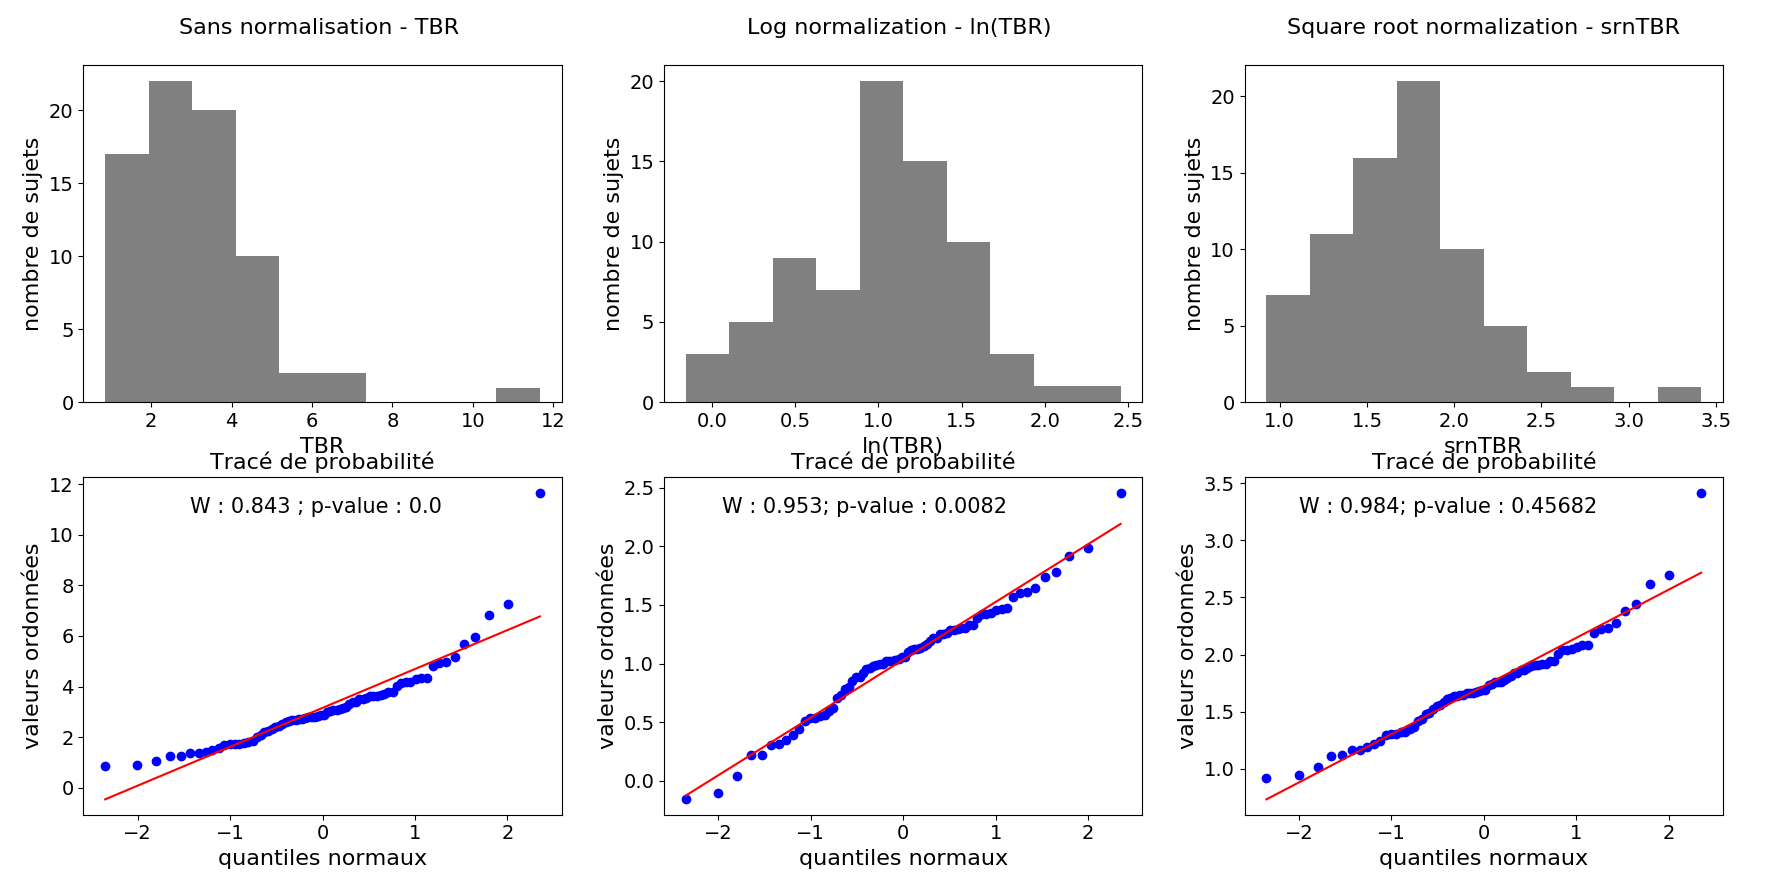
\includegraphics[width=1.0\linewidth]{figures/chapter-4/tbr-normalization} 
  \caption[Comparaison de techniques de normalisation des valeurs de \gls{tbr}.]{Comparaison de techniques de normalisation des valeurs de \gls{tbr}. 
	Les histogrammes des distributions de valeurs \gls{tbr} non nomalisées,
	log normalisées et \textit{square-root} normalisées sont presentés à la première ligne. La seconde ligne contient les tracés de probabilités comparant les
	dstributions. La statistique W du test de Shapiro-Wilk et la $p$-value correspondante sont affichées sur chaque tracé de probabilité.}
  \label{Figure:tbr_normalization}
\end{figure}

Les \gls{tbr} sont donc normalisés suivant l'équation suivante :
\begin{equation}
\label{eq:tbr_srntbr_computation}
\text{srnTBR} = \sqrt{ \text{max}(\frac{\bar{P}_{Fz,\theta}}{\bar{P}_{Fz,\beta} } ; \frac{\bar{P}_{Cz,\theta}}{\bar{P}_{Cz,\beta}} ) }.
\end{equation}

\subsection{Méthodes de partitionnement de la distribution des Theta-beta ratios} \label{clustering}

Afin de déterminer s'il existe un groupe d'enfants \gls{tdah} présentant un \gls{tbr} élevé, trois méthodes de partitionnement, issues de familles différentes,
sont appliquées aux \gls{srntbr} : 
\begin{itemize}
\item une qui se base sur les distributions Gaussiennes (\glsfirst{gmm} et \glsfirst{bgmm}), 
\item une sur les distances (la méthode de Ward),
\item et une autre sur les densités (\glsfirst{dbscan}). 
\end{itemize}

Ces méthodes ont été choisies car elles s'appuient sur des critères différents afin de déterminer s'il existe bien deux groupes d'enfants \gls{tdah}. Il a été décidé
d'avoir recours à trois méthodes pour pouvoir comparer les résultats de chacune d'entre elles et de déterminer s'ils sont fiables ou non. Davantage de méthodes auraient pu
être utilisées, cependant le message aurait été complexifié.   

Les analyses statistiques sont effectuées avec la bibliothèque Python Scikit Learn (v0.18.1, \citet{Pedregosa2011}).

\subsubsection{Partitionnement basé sur les distributions : \gls{gmm} et \gls{bgmm}} 
Un \textit{mixture model} est un modèle probabiliste qui permet d'identifier la présence de sous-populations dans une population. Un \textit{mixture model}
correspond à une \textit{mixture distribution} qui représente la distribution de probabilités des observations dans la totalité d'une population.
La distribution des \gls{srntbr} est ainsi tracée et ajustée par un \gls{bgmm} puis par un \gls{gmm} pour comparaison \citep{Attias2000, Blei2006}. 

Un \textit{Gaussian Mixture Model} est un modèle qui suppose que toutes les observations proviennent d'un mélange 
d'un nombre fini de distributions Gaussiennes aux paramètres inconnus \citep{Yu2016}. 
Le \gls{bgmm}, à la différence du \gls{gmm}, utilise des \textit{a priori} sur la distribution des données pour 
assigner des probabilités \textit{a posteriori} à chaque \textit{Gaussian Mixture} distribution. Un grand nombre de \gls{tbr} 
extraits de sujets sains de la base de données \gls{cmi-hbn} étant disponible, ces valeurs sont donc utilisées pour estimer les \textit{a priori} du \gls{bgmm}. 
Lorsque les observations sont ajustées par un \gls{bgmm} ou un \gls{gmm}, un modèle gaussien constitué d'un nombre prédéfini de courbes Gaussiennes est 
créé pour modéliser les données. Ici, la distribution multi-modale des valeurs de \gls{srntbr} est modélisée par un \gls{bgmm} avec un nombre 
de modes/composantes allant de 1 à 3. 
Il en va de même pour l'algorithme du \gls{gmm}. 

Il a été décidé d'avoir recours à un nombre de composantes variant entre 1 et 3 pour pouvoir valider ou infirmer l'hypothèse qu'il existe deux groupes d'enfants \gls{tdah}.
En effet, le modèle à une composante va être comparé à celui à deux composantes, et celui à deux le sera à celui à trois composantes afin de déterminer quel modèle 
représente le mieux la distribution des \gls{srntbr}. 

Pour un \gls{gmm} avec $K$ composantes, la $k^{th}$ composante a une moyenne de $\mu_k$ et une variance de $\sigma_k$ dans le cas univarié. Les poids associés $\Phi_k$ aux composantes
$C_k$ sont définis tels que $\sum_{i=1}^{K} \Phi_i = 1$ pour que la distribution de probabilité totale soit égale à 1. Mathématiquement un \gls{gmm} se traduit ainsi \citep{Santosh2013} :
\begin{equation}
\label{eq:tbr_gmm_univariate}
p(x) = \sum_{i=1}^{K} \Phi_i\mathcal{N}( x | \mu_i, \sigma_i),
\end{equation}

avec :

\begin{equation}
\label{eq:tbr_gaussian}
\mathcal{N}( x | \mu_i, \sigma_i) = \frac{1}{\sigma_i\sqrt{2\pi}} \text{exp}\Big(-\frac{(x - \mu_i)^2}{2\sigma_i^2}\Big).
\end{equation}

Si le nombre de composantes $K$ est connu, la technique d'\gls{em} est la plus couramment utilisée pour estimer les paramètres du \textit{mixture model}. L'algorithme d'\gls{em}
cherche à maximiser la probabilité, ou \textit{likelihood}, des données observéees étant donné les paramètres du modèle. Dans le cas des \textit{mixture models}, l'\gls{em}
consiste en deux étapes :
\begin{enumerate}
\item Etape d'\textit{expectation} : calcul de l'\textit{expectation} de la composante $C_k$ pour chaque point $x_i \in X$ étant donné les paramètres du modèle $\Phi_k$, $\sigma_k$,
et $\mu_k$. L'\textit{expectation} correspond à la probabilité qu'$x_i$ soit généré par la composante $C_k$,
\item Etape de \textit{maximization} : maximisation des \textit{expectations} calculées à la première étape afin de mettre à jour les valeurs $\Phi_k$, $\sigma_k$,
et $\mu_k$. 
\end{enumerate}

Ce processus est répété jusqu'à ce que l'algorithme converge, menant à l'estimation de la \textit{maximum likelihood}. La même approche est suivie pour le \gls{bgmm} pour lequel 
les informations des \textit{a priori} sont intégrées. 

Afin de déterminer le nombre de composantes qui décrit le mieux la distribution des \gls{srntbr}, la significativité de la différence entre chaque 
modèle est testée grâce à un test $\chi^2$ sur la déviance \citep[Chapitre~6]{James2013}. Etant donné que dans le cas du \textit{Gaussian Mixture Model} les modèles
sont imbriqués, c'est à dire que le deuxième modèle peut être obtenu en imposant des contraintes sur le premier modèle, le test de 
deviance est adapté. La déviance est une mesure de la qualité de l'ajustement (\textit{goodness-of-fit} 
en anglais) d'un modèle statistique et est définie comme suit :
\begin{equation}
\label{eq:tbr_deviance}
\text{D} = -2(log(L(\beta_{0})) - log(L(\beta_{\alpha}))),
\end{equation}
où $log(L(\beta_{0}))$ est la \textit{log likelihood} du modèle nul et $log(L(\beta_{\alpha}))$ est la \textit{log likelihood} du modèle alternatif. 
La \textit{log likelihood} a pour rôle de donner une idée sur la capacité des données à résumer les paramètres de la distribution de probabilités. 
La multiplication par -2 est une étape nécessaire pour convertir la \textit{log likelihood} en une distribution \textit{chi-square} qui permet 
l'utilisation d'un test $\chi^2$ pour tester la significativité statistique. Le seuil de significativité est fixé à $\alpha = 0.01$.

\subsubsection{Partitionnement basé sur les distances : méthode de Ward}
La méthode de Ward est un critère utilisé pour rassembler deux partitions lors d'un partitionnement hiérarchique agglomérant (\textit{hierarchical agglomerative clustering} 
en anglais) \citep{Ward1963}. Ce type d'algorithme de partitionnement fusionne de façon récursive deux groupes similaires, qui initiallement ne comportent qu'une seule observation, jusqu'à obtenir une
grande partition comprenant l'ensemble des données \citep[Chapitre~10]{James2013}.

Un exemple schématique de ce type de partitionnement est représenté à la Figure~\ref{Figure:tbr_hierarchical_agglomerative_clustering_example} avec six observations (A, B, C, D, E, F) :
\begin{enumerate}
\item \emph{Première étape :} calcul de la proximité des points individuels qui sont considérés comme des groupes,
\item \emph{Deuxième étape :} fusion des groupes similaires pour en former de nouveaux. Sur la Figure~\ref{Figure:tbr_hierarchical_agglomerative_clustering_example}, B et C d'une part et D et E
d'autre part sont des groupes similaires et sont donc fusionnés. Il reste désormais quatre groupes : A, BC, DE et F,
\item \emph{Troisième étape :} nouveau calcul de la proximité entre les groupes restants et fusion de ceux qui sont similaires pour en obtenir de nouveaux : A, BC, DEF,
\item \emph{Quatrième étape :} nouveau calcul de la proximité entre les nouveaux groupes et fusion de ceux qui sont similaires ce qui conduit à deux groupes : A, BCDEF,
\item \emph{Cinquième étape :} les deux groupes sont fusionnés pour en former un unique.
\end{enumerate}

\begin{figure}[h!]
  \centering
	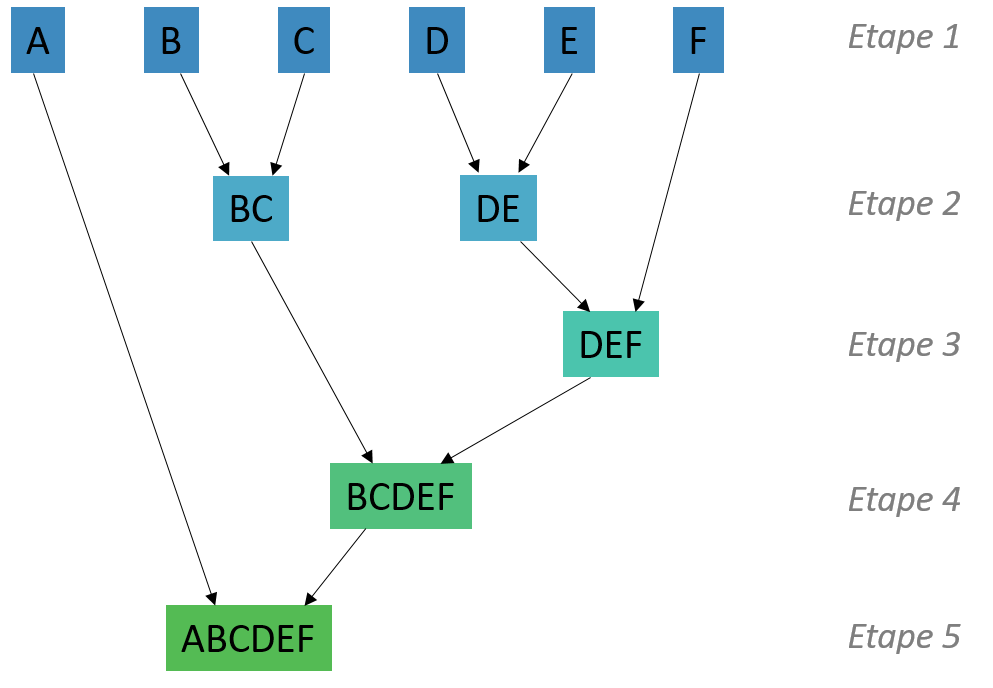
\includegraphics[width=0.7\linewidth]{figures/chapter-4/tbr-hierarchical-agglomerative-clustering-example} 
  \caption[Exemple schématique des étapes de \textit{hierarchical agglomerative clustering}.]{Exemple schématique des étapes de \textit{hierarchical agglomerative clustering} sur six observations : A, B, C, D, E, F.} 
	\label{Figure:tbr_hierarchical_agglomerative_clustering_example} 
\end{figure}

Plusieurs méthodes existent pour quantifier la proximité de deux partitions, ici on se base sur la méthode de Ward qui minimise 
la variance des deux groupes qui sont fusionnés \citep{Ward1963}.

Le nombre de groupes estimé par cette méthode varie de 2 à 3 pour comparer les résultats obtenus à ceux du \gls{bgmm}. 

Ce partionnement hierarchique agglomérant est représenté par un dendrogramme, dont un exemple est donné à la 
Figure~\ref{Figure:tbr_dendrogram_example}. Il s'agit d'un arbre souvent renversé dont l'analyse visuelle 
peut aider à choisir le nombre de partitions à identifier \citep[Chapitre~10]{James2013}.
Chaque feuille de l'arbre correspond à une observation et, plus on remonte dans l'arbre, plus les feuilles se regroupent en branches lorsque elles 
sont similaires. Ensuite, les branches fusionnent avec d'autres branches ou feuilles similaires. Plus la fusion entre deux groupes a lieu tôt, c'est à dire en bas de
l'arbre, plus ceux-ci se ressemblent. La similitude entre deux groupes est mise en évidence par l'axe des ordonnées de l'arbre :
plus le trait vertical d'un dendrogramme est grand, plus les groupes fusionnés sont différents. Ici l'axe des ordonnées correspond à la distance de Ward.

Afin de se donner une idée du nombre de groupes à identifier, des lignes horizontales coupant les lignes verticales du dendrogramme peuvent être
tracées : le nombre de ligne verticales coupées correspond au nombre de groupes comme illustré à la Figure~\ref{Figure:tbr_dendrogram_example}.
Le plus souvent, il est choisi de tracer les lignes horizontales de façon à ce qu'elles coupent les plus longs traits verticaux du dendrogramme, 
toutefois un tel choix peut manquer de précision \citep[Chapitre~10]{James2013}.

\begin{figure}[h!]
  \centering
	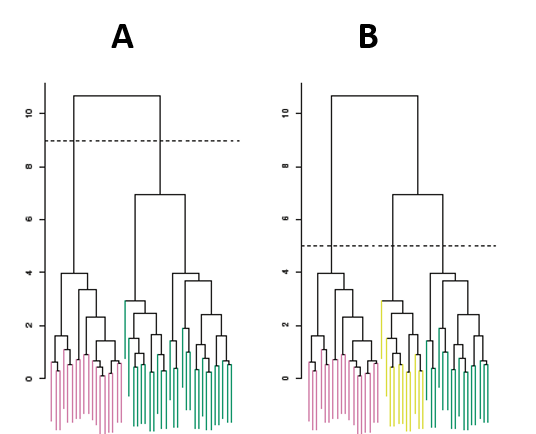
\includegraphics[width=0.7\linewidth]{figures/chapter-4/tbr-dendrogram-example} 
  \caption[Exemples de dendrogrammes obtenus lors d'un partitionnement hiérarchique.]{Exemples de dendrogrammes 
	issus de \citet[Chapitre~10]{James2013} obtenus lors d'un partitionnement hiérarchique. En \textbf{A}, le dendrogramme est coupé
	par une ligne horizontale (en pointillés noirs) à une hauteur de 9 ce qui conduit à deux groupes (un rose et un vert). En \textbf{B}, le dendrogramme
	est coupé à une hauteur de 5 menant cette fois-ci à trois groupes (en rose, jaune et vert).} 
	\label{Figure:tbr_dendrogram_example} 
\end{figure}

\subsubsection{Partitionnement basé sur les densités : \gls{dbscan}}
\gls{dbscan} est un algorithme de partitionnement de données qui s'appuie sur la densité des partitions estimées \citep{Ester1996}. 
Deux paramètres sont nécessaires pour permettre à l'algorithme de partitionner la donnée : la distance $\epsilon$ et le nombre minimum de points 
$MinPts$ devant se trouver dans un rayon $\epsilon$ pour que ces points forment un groupe.
 
Pour un point donné, l'algorithme récupère son voisinage dans un rayon $\epsilon$ et vérifie qu'il contient bien au moins $MinPt$s points, auquel cas, 
ce point est alors considéré comme faisant partie d'un groupe. On parcourt ensuite le voisinage 
dans un rayon $\epsilon$ de proche en proche afin de trouver l'ensemble des points du groupe.

Afin de choisir les valeurs des paramètres $\epsilon$ et $MinPts$, la topologie de l'espace à partitionner est à prendre en compte. En effet, une 
trop faible valeur de $\epsilon$  et/ou une trop grande valeur de$MinPts$ peuvent empêcher 
l'algorithme de propager les partitions. A l'inverse, une trop grande valeur pour $\epsilon$  
et/ou une trop faible valeur pour $MinPts$ peuvent conduire l'algorithme à ne renvoyer que du bruit. 
 
Ici, $MinPts$ est déterminé grâce une méthode heuristique \citep{Birant2007} :
\begin{equation}
\label{eq:tbr_dbscan}
MinPts = ln(\text{n}),
\end{equation}
avec n le nombre total de points à être partitionnés.

Une méthode pour déterminer la valeur $\epsilon$ optimale est de tracer le graphique des \textit{k-distance} obtenu par la méthode des k plus proches voisins 
(\gls{knn} en anglais) non supervisée en prenant k $= MinPts$ \citep{Goldberger2005, Ester1996}. Le principe de cette méthode
est de trouver un nombre prédéfini d'observations, noté k, les plus proches en distance (ici de Minkowski) d'un nouveau point et de prédire la classe de ce dernier. 

Le graphique des distances k (\textit{k-distance plot} en anglais) représente les distances de chaque observation à son voisin le plus éloigné 
lors du partitionnement par \gls{knn}. Les distances obtenues sont ensuite classées par ordre décroissant. 
Ainsi, étant donné que les points bruités sont censés avoir une \textit{k-distance} bien plus élevée que celle des autres points, on peut 
s'attendre à observer un changement de pente, un "coude", sur ce tracé : l'ordonnée de ce point, déterminée visuellement, correspond à $\epsilon$. Un \textit{k-distance plot}
obtenu sur des données factices est présenté à la Figure~\ref{Figure:tbr_k_distance_plot_example} pour illustrer comment est déterminé $\epsilon$. 

\begin{figure}[h!]
  \centering
	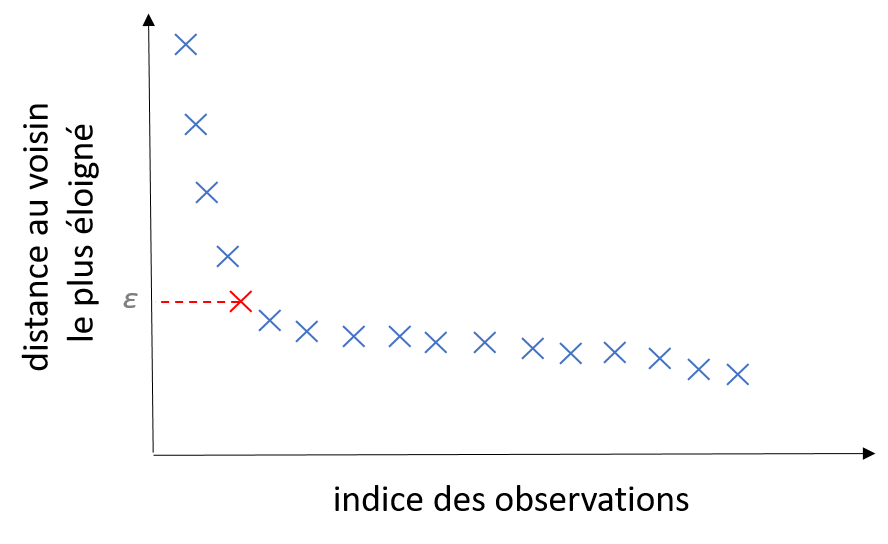
\includegraphics[width=0.7\linewidth]{figures/chapter-4/tbr-k-distance-plot-example} 
  \caption[Exemple de \textit{k-distance plot} sur des données factices.]{Exemple de \textit{k-distance plot} sur des données factices. Les observations 
	ayant une \textit{k-distance} élevée sont potentiellement
	des outliers. L'observation représentée par une croix rouge correspond au "coude" dont l'abscisse correspond à $\epsilon$.} 
	\label{Figure:tbr_k_distance_plot_example} 
\end{figure}

Le \textit{silhouette coefficient} est utilisé pour rendre compte de la qualité du partitionnement : -1 est la pire valeur, 1 la meilleure et 0
correspond à des groupes qui se superposent.

\subsection{Identification du seuil optimal pour la personnalisation du protocole de Neurofeedback}

Les seuils de discrimination obtenus lorsque les méthodes présentées précédemment identifient deux groupes parmi la population d'enfants \gls{tdah} 
sont comparés entre eux, notamment à l'aide d'une courbe \gls{roc}, afin de déterminer le seuil \gls{tbr} à utiliser pour personnaliser le protocole de \gls{nfb}. 

\subsubsection{Seuil obtenu par le \gls{bgmm}}
Si le \gls{bgmm} à deux composantes est identifié comme offrant le meilleur ajustement du modèle, la distribution théorique de chaque composante 
est utilisée pour en déduire la valeur du seuil conduisant à la meilleure discrimination entre les deux groupes. 

Ce seuil correspond à l'abscisse $x$ de l'intersection des deux Gaussiennes, c'est à dire qu'il faut trouver $x$ tel que $G_1(x) = G_2(x)$, avec $G_1$ et $G_2$ les deux Gausiennes estimées. 
Pour déterminer $x$ il suffit de traduire mathématiquement les deux Gaussiennes ce qui
conduit à une équation quadratique dont les coefficients comportent les moyennes et variances de ces deux distributions.

\subsubsection{Tracé de la courbe \gls{roc} obtenue grâce au \gls{bgmm} à deux composantes}
Une courbe \gls{roc} est ensuite tracée à partir du \gls{bgmm} à deux composantes, c'est à dire qu'on se base sur les résultats de ce partitionnement pour déterminer les 
vrais positifs et vrais négatifs (ceux qui sont assignés à la bonne classe) et les faux positifs et faux négatifs (ceux qui sont assignés à la mauvaise classe). 

Habituellement, une courbe \gls{roc}
est obtenue grâce à un \textit{gold standard} qui provient de résultats cliniques, alors qu'ici le partionnement retourné par le \gls{bgmm} à deux composantes est utilisé : on suppose 
que ces deux groupes existent et sont correctement estimés par cette méthode, et c'est à partir de ces résultats que la capacité à discriminer les patients \gls{tdah} est évaluée.

Une représentation graphique des résultats factices d'un \gls{bgmm} à deux composantes est présentée à la Figure~\ref{Figure:tbr_bgmm_example} : les deux Gaussiennes obtenues correspondent 
aux deux groupes supposés correctement estimés,
le seuil calculé pour le \gls{bgmm} à deux composantes est représenté par la droite verticale noire, les populations de vrais positifs et négatifs ainsi que celles des faux positifs 
et négatifs sont également spécifiées. 

\begin{figure}[h!]
  \centering
	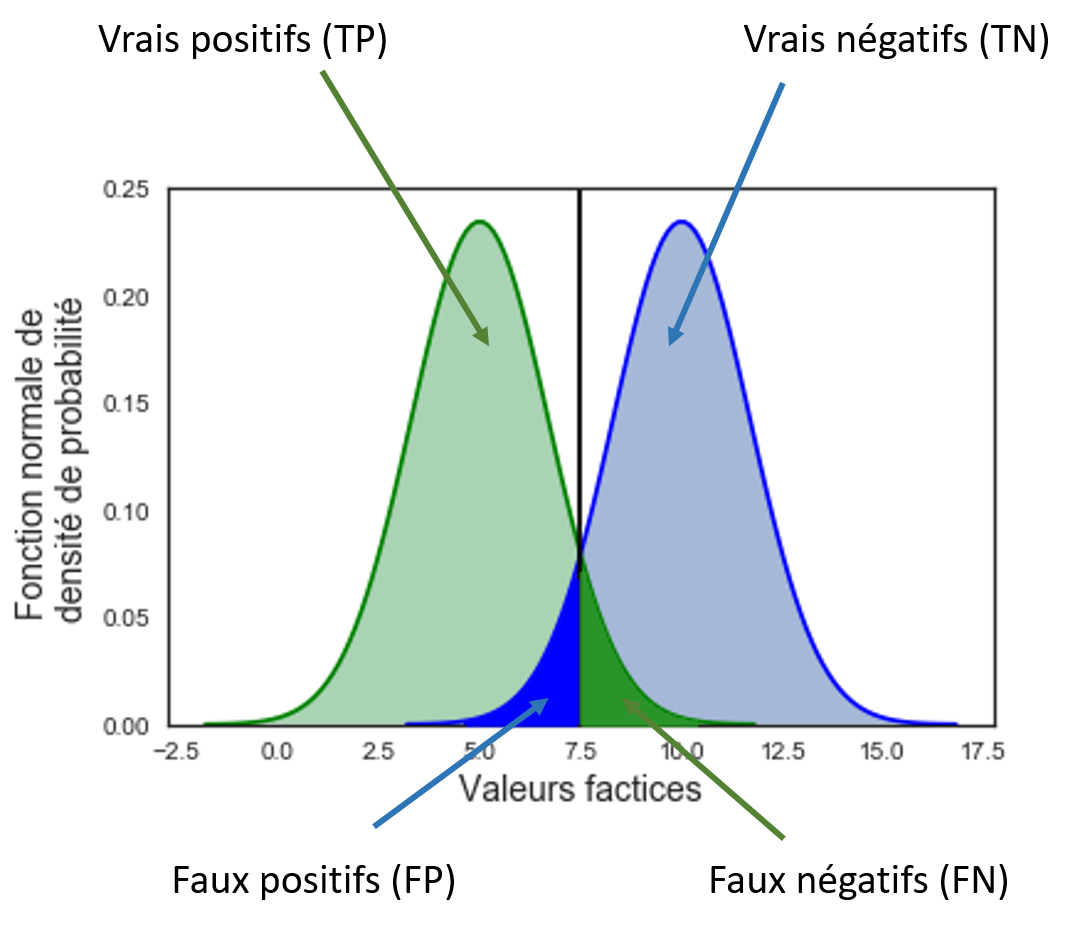
\includegraphics[width=0.7\linewidth]{figures/chapter-4/tbr-bgmm-example} 
  \caption[Tracés des résultats factices d'un \gls{bgmm} à deux composantes.]{Tracés des résultats factices d'un \gls{bgmm} à deux composantes. Les deux Gaussiennes estimées en vert et bleu correspondent aux deux groupes délimités par la droite
	verticale noire. En supposant que ces groupes sont correctement estimés, les populations de vrais positifs et négatifs et faux positifs et négatifs sont représentées.} 
	\label{Figure:tbr_bgmm_example} 
\end{figure}

La courbe \gls{roc} correspondant à ce modèle est obtenue en faisant varier le seuil de discrimination, ainsi le taux de faux positifs (\gls{fpr} en anglais) 
et celui de vrais positifs (\gls{tpr} en anglais), qui sont respectivement les abscisses et les ordonnées de la courbe \gls{roc}, 
vont évoluer \citep[Chapitre~4]{James2013} : 

\begin{equation}
\label{eq:tbr_fpr_tpr}
\text{FPR} = \frac{\text{FP}}{\text{FP + TN}} = 1 - \text{TNR},
\end{equation}

\begin{equation}
\label{eq:tbr_tpr}
\text{TPR} = \frac{\text{TP}}{\text{TP + FN}} = 1 - \text{FNR},
\end{equation}
où FP est le nombre de vrais positifs, TN le nombre de vrais négatifs, TP le nombre de vrais positifs et FN le nombre de faux négatifs. 
TNR est le taux de vrais négatifs et FNR le taux de faux négatifs.
De plus, FP $+$ TN correspond au nombre total de négatifs, et TP $+$ FN au nombre total de positifs.

Les courbes \gls{roc} sont fréquemment utilisées pour mesurer la performance de partitionnements binaires, notamment grâce à
l'\gls{auc} : plus cette aire est grande, plus la courbe \gls{roc} s'éloigne du partitionnement aléatoire modélisé par une droite allant
de (0, 0) à (1, 1) \citep[Chapitre~3]{James2013}. 

\subsubsection{Comparaison des seuils identifiés par les méthodes de partitionnement}
Les seuils identifiés pour la discrimination de deux groupes par le \gls{gmm}, la méthode de Ward et le \gls{dbscan} sont comparés à celui trouvé pour 
le \gls{bgmm} à deux composantes en étant ajoutés à la courbe \gls{roc} et grâce à une métrique quantifiant la précision de ces seuils, 
il s'agit de la justesse (\gls{acc} en anglais) :

\begin{equation}
\label{eq:tbr_accuracy}
\text{ACC} = \frac{\text{TP + TN}}{\text{TP + TN + FP + FN}}.
\end{equation}

Enfin, les seuils de \gls{tbr} calculés dans cette étude sont également comparés à ceux utilisés dans la littérature. Les seuils de 5 et de 4.5 sont
ajoutés à la courbe \gls{roc} car \citet{Kerson2013} ont suggéré l'utilisation d'un seuil de \gls{tbr} à 5, même si lors de leur étude clinique il a été fixé 
à 4.5 (NCT02251743, Arnold, Ohio State University, ClinicalTrials.gov) tout comme le seuil utilisé pendant l'étude NEWROFEED. 

Le seuil qui sépare 35\% des valeurs de 
\gls{tbr} est également ajouté à la courbe \gls{roc} pour visualiser les résultats de \citet{Zhang2017} basés sur les conclusions de \citet{Clarke2011}.
De plus, le seuil conduisant à 10\% de \gls{fpr} selon le partitionnement par le \gls{bgmm} à deux composantes est aussi ajouté à la courbe \gls{roc}. 
En effet, un seuil menant à un faible \gls{fpr} est intéressant pour idéalement traiter les patients qui appartiennent au sous-groupe \gls{tbr} élevé avec 
un protocole adapté à leur profil \gls{eegi}, comme la diminution du \gls{tbr}.

\section{Partitionnement de la distribution des Theta-Beta ratios}

Les \gls{tbr} ont été extraits en suivant les étapes présentées en \ref{extraction_tbr}. Les \gls{srntbr} calculés sont ensuite partitionnés à l'aide de trois
méthodes (\gls{bgmm}, partitionnement hiérarchique et \gls{dbscan}) et les seuils de séparation obtenus pour chacune de ces méthodes, dans le cas où deux classes sont 
identifiées, sont comparés entre eux.  

\subsection{Partitionnements obtenus}

Les différentes méthodes décrites précédemment sont appliquées tour à tour sur l'ensemble des \gls{srntbr}.

\subsubsection{Bayesian Gaussian Mixture Model}

Les résultats des \gls{bgmm} avec un nombre de composantes allant de 1 à 3 sont représentés à la Figure~\ref{Figure:tbr_bgmm}. 

\begin{figure}[h!]
  \centering
	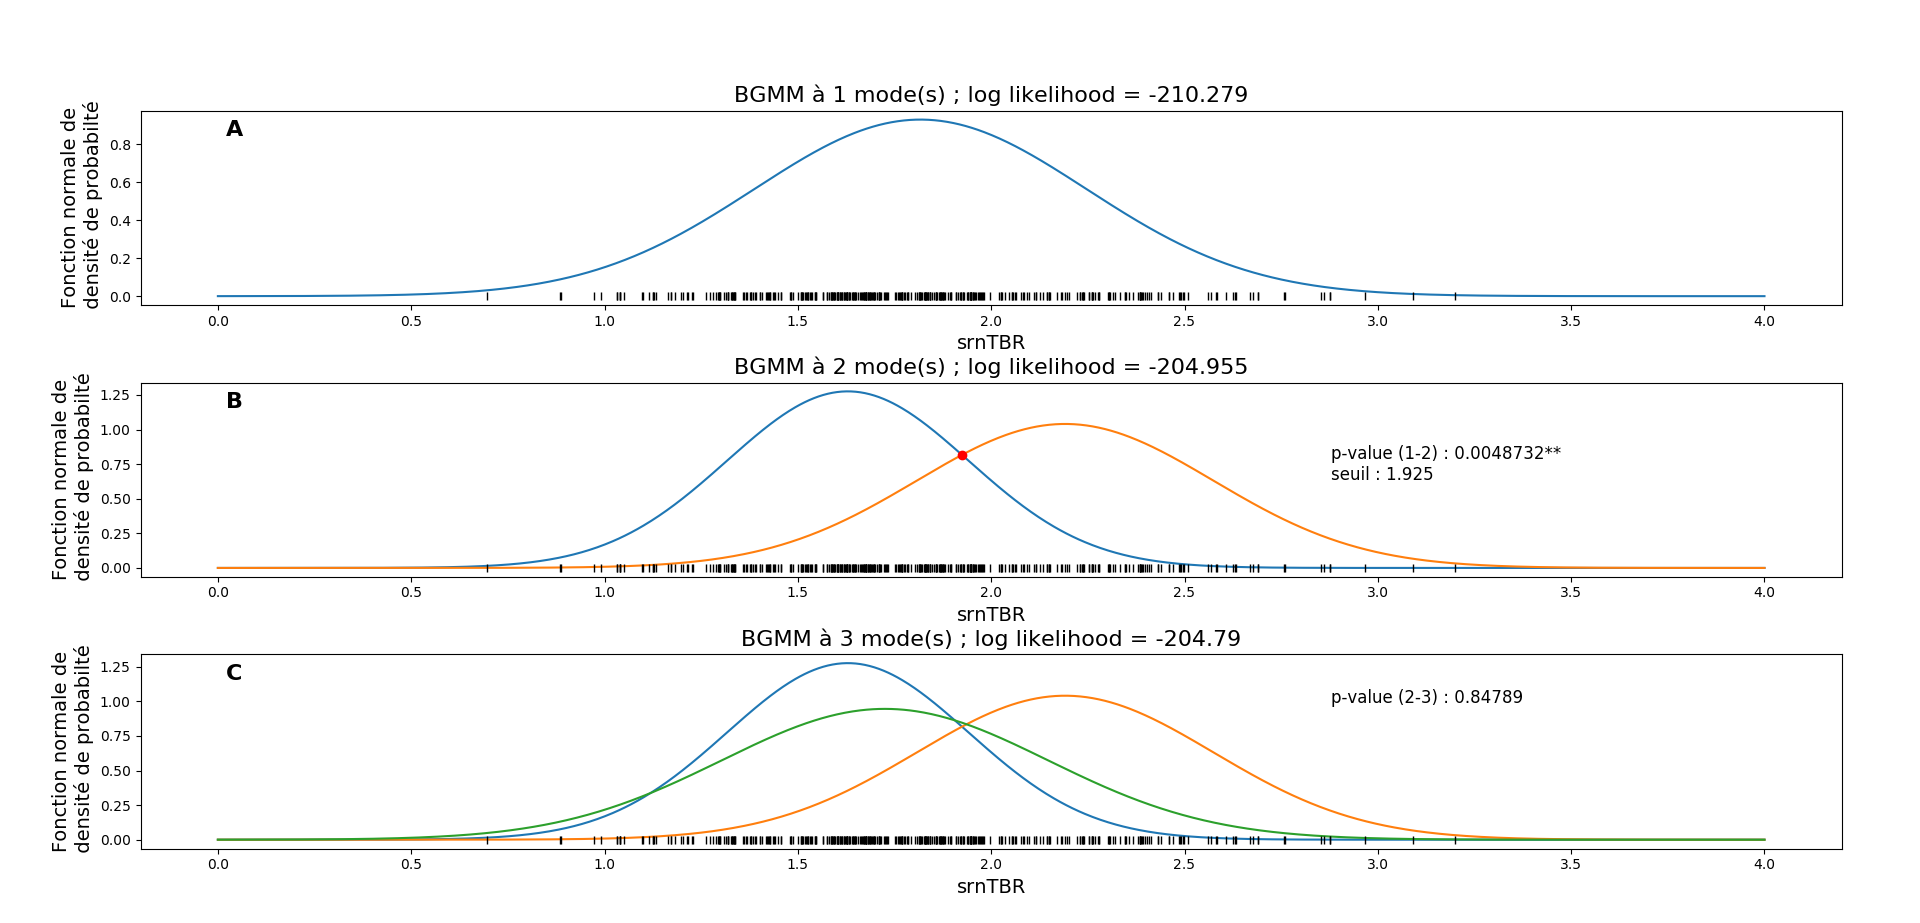
\includegraphics[width=1.0\linewidth]{figures/chapter-4/tbr-bgmm} 
  \caption[Résultats des \gls{bgmm} avec une à trois composantes.]{Tracés des distributions de \gls{srntbr} (\textit{rug plot}) avec en \textbf{A} 1 mode, en \textbf{B} 
	2 modes et en \textbf{C} 3 modes du \gls{bgmm} superposés. $P$-value (1-2) correspond
	à la $p$-value du test de déviance comparant les \gls{bgmm} à 1 mode et 2 modes ; $p$-value (2-3) correspond à la $p$-value du test de déviance comparant les \gls{bgmm}
	à 2 modes et 3 modes. La significativité est symbolisée par ** et fixée à 1\%. Le seuil \gls{srntbr} est précisé pour le modèle à 2 composantes et représenté par un cercle bleu.}
  \label{Figure:tbr_bgmm} 
\end{figure}

Une différence statistiquement significative est observée dans la modélisation des distributions entre les modèles à 1 (modèle nul) et à 2 composantes 
du \gls{bgmm} ($p$-value = 0.005), alors qu'aucune différence statistiquement significative n'est observée entre les modèles à 2 (modèle nul) 
et à 3 composantes du \gls{bgmm} ($p$-value = 0.850). On peut donc en conclure que le \gls{bgmm} à 2 modes décrit mieux la donnée que les deux
autres modes. 

Le \gls{gmm} arrive à la même conclusion : la distribution des \gls{srntbr} semble bimodale ($p$-value pour la comparaison
entre le modèle à 1 mode (modèle nul) et à 2 modes = 0.002). Ainsi, les \textit{a priori} utilisés pour le \gls{bgmm} semblent bien 
représenter la donnée. 

\subsubsection{Méthode de Ward}
Tout d'abord, les résultats d'un partitionnement hiérarchique agglomérant basé sur la distance de Ward sont représentés sur le dendrogramme présenté à la 
Figure~\ref{Figure:tbr_ward_dendrogram}. 

\begin{figure}[h!]
  \centering
	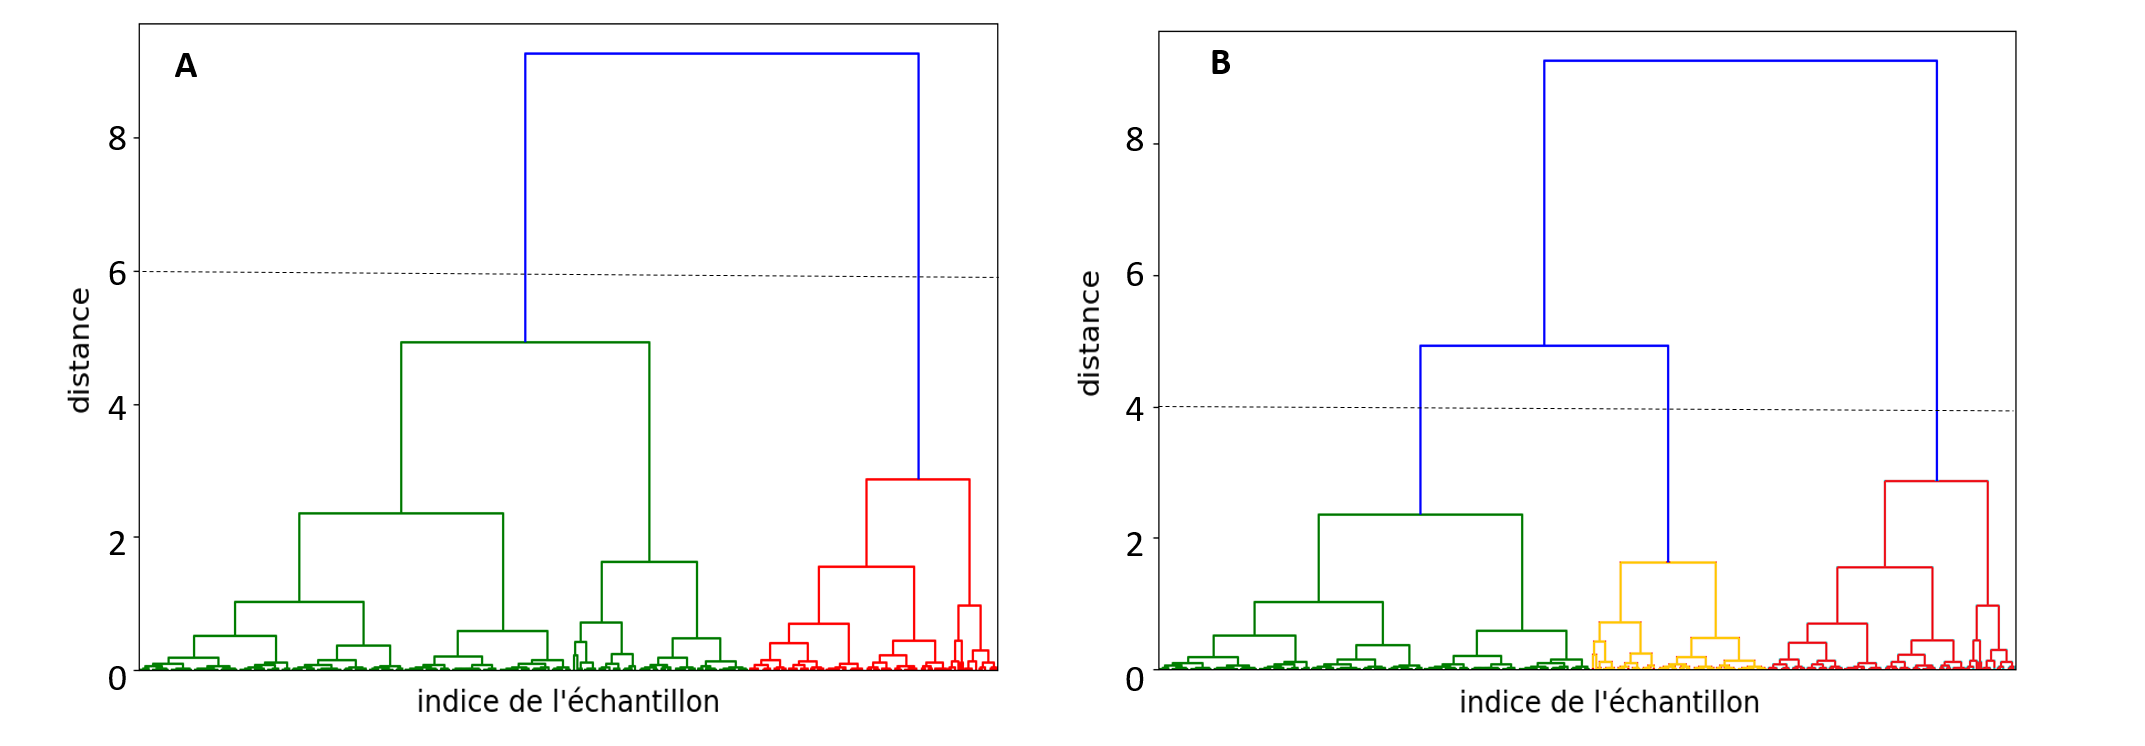
\includegraphics[width=1\linewidth]{figures/chapter-4/tbr-dendrogram-ward} 
  \caption[Dendrogrammes représentant le partitionnement obtenu suivant la méthode de Ward.]{Dendrogrammes représentant le partitionnement obtenu suivant 
	la méthode de Ward. En \textbf{A}, tous les liens connectant des noeuds 
	avec des distances plus grandes ou égales à un seuil fixé à 6 (représenté en pointillés noirs) sont colorés en bleu, ce qui mène à deux groupes	
	(un vert et un rouge). En \textbf{B}, le seuil est fixé à 4, conduisant à trois partitions.}
  \label{Figure:tbr_ward_dendrogram}
\end{figure}

Cette représentation permet de supposer que les données pourraient être séparées en 2 groupes (en rouge et vert) 
mais aussi en 3 (en vert, rouge et orange). Les résultats d'un partitionnement en 2 et 3 groupes sont représentés 
à la Figure~\ref{Figure:tbr_ward_histograms} sous forme d'histogrammes.

\begin{figure}[h!]
  \centering
	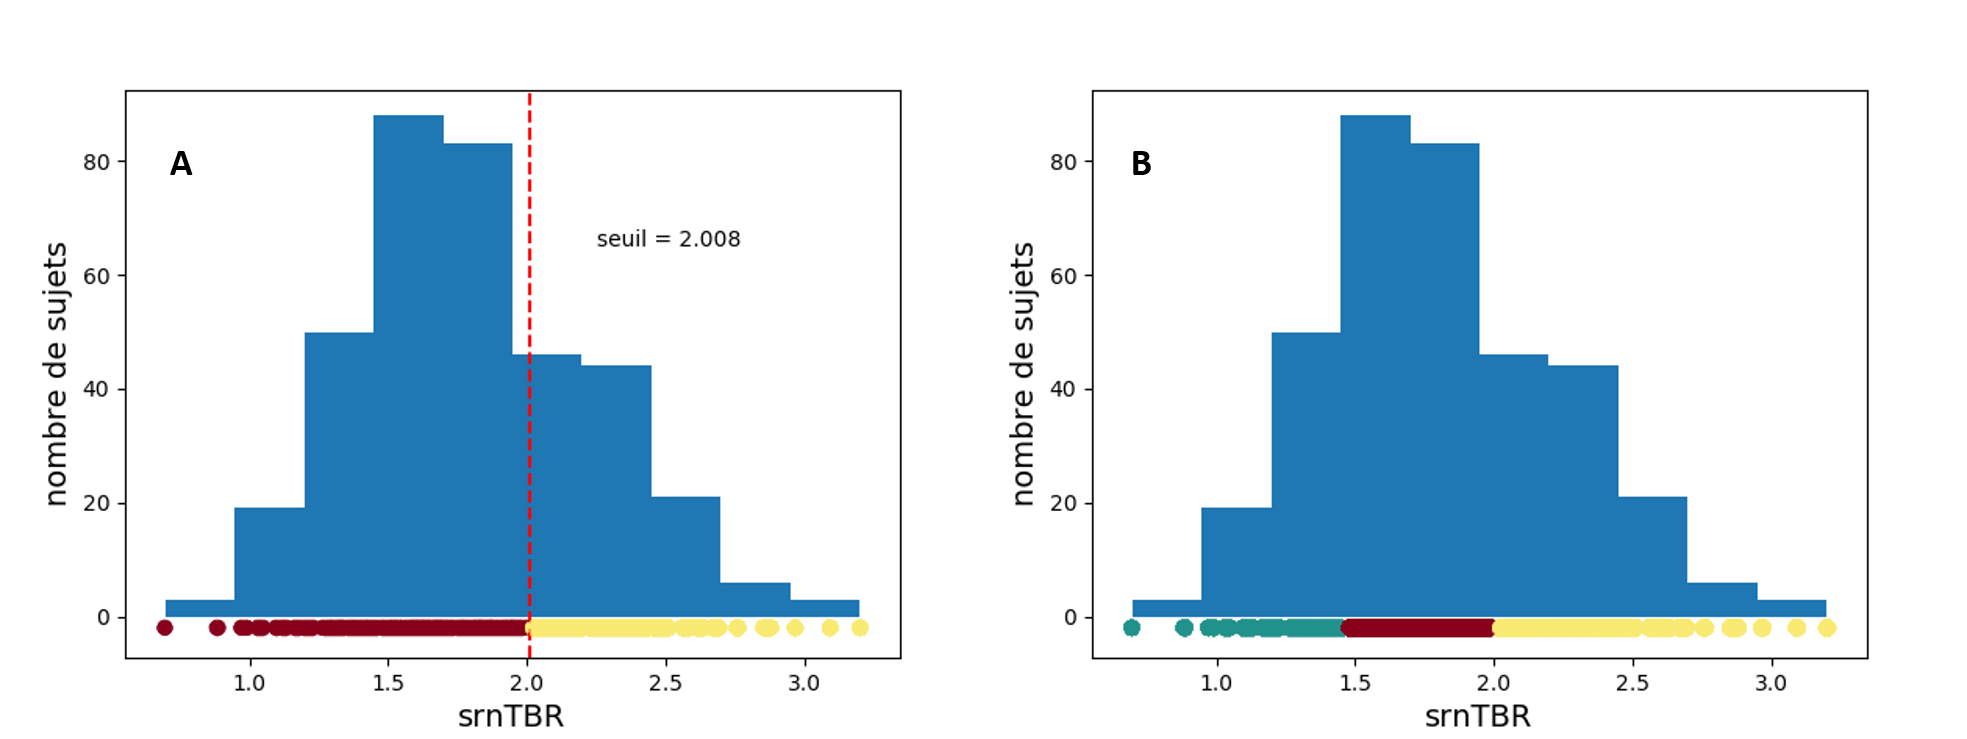
\includegraphics[width=1.0\linewidth]{figures/chapter-4/tbr-histogram-ward} 
  \caption[Résultats du partitionnement en deux et trois groupes selon la méthode de Ward.]{Distribution des \gls{srntbr} répartis grâce à la méthode de Ward en \textbf{A} : 2 groupes (vert et rouge) et \textbf{B} : 3 groupes 
	(vert, rouge et orange). Le seuil séparant la distribution des \gls{srntbr} en deux groupes est représenté par la ligne verticale en pointillés bleus sur la 
	figure \textbf{A}.}
  \label{Figure:tbr_ward_histograms}
\end{figure}

Dans le cas du partitionnement en 3 groupes, le groupe des \gls{srntbr} élevés est toujours identifié (en rouge), le troisième groupe est formé dans 
la sous population des \gls{srntbr} plus faibles. 

\subsubsection{DBSCAN}

Les paramètres $MinPts$ et $\epsilon$ de l'algorithme \gls{dbscan} sont tout d'abord déterminés. Etant donné qu'ici $MinPts = 6$, 
l'algorithme des \gls{knn} prend $k = 6$ : on obtient alors le graphique des distances k présenté à la Figure~\ref{Figure:tbr_dbscan_kdistance_plot}, 
où un coude est observé à $y = 0.048$. Cette valeur, identifiée visuellement, est choisie pour $\epsilon$.

\begin{figure}[h!]
  \centering
	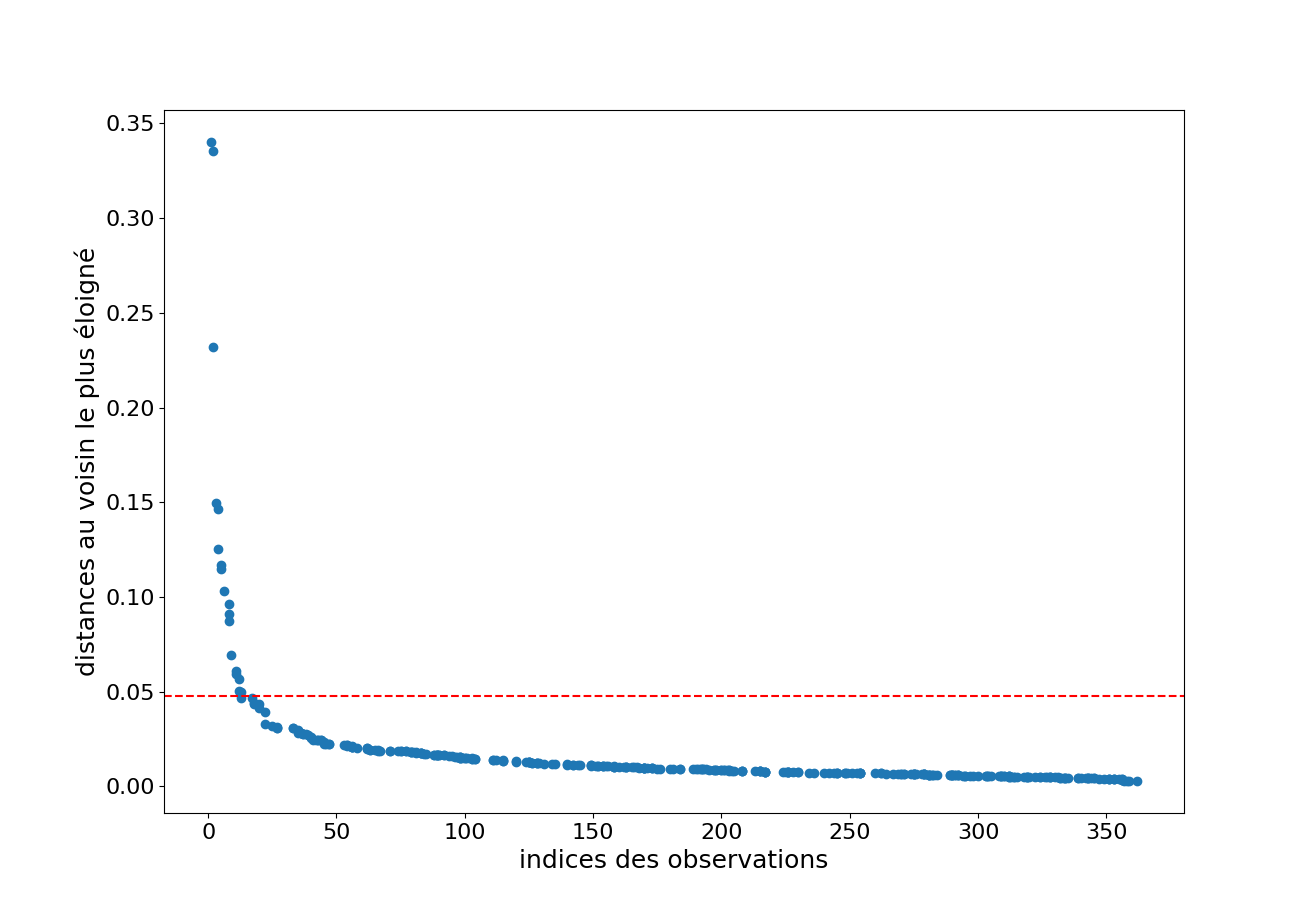
\includegraphics[width=0.7\linewidth]{figures/chapter-4/tbr-dbscan-knn-plot} 
  \caption[Graphique des k distances pour la méthode \gls{dbscan}.]{Graphique des k distances pour la méthode \gls{dbscan}. La ligne en pointillés noirs coupe la courbe où le coude est identifié.}
  \label{Figure:tbr_dbscan_kdistance_plot}
\end{figure}

Le partitionnement par \gls{dbscan} est représenté à Figure~\ref{Figure:tbr_dbscan_clustering_plot} : deux groupes (en rouge et vert) et 13 
points considérés comme du bruit et donc attribués à aucun groupe (en noir) sont identifiés. Le \textit{silhouette coefficient} de $\text{s} = 0.388$
indique un partitionnement convenable, car beaucoup plus grand que -1, mais dont les groupes sont proches l'un de l'autre. 

\begin{figure}[h!]
  \centering
	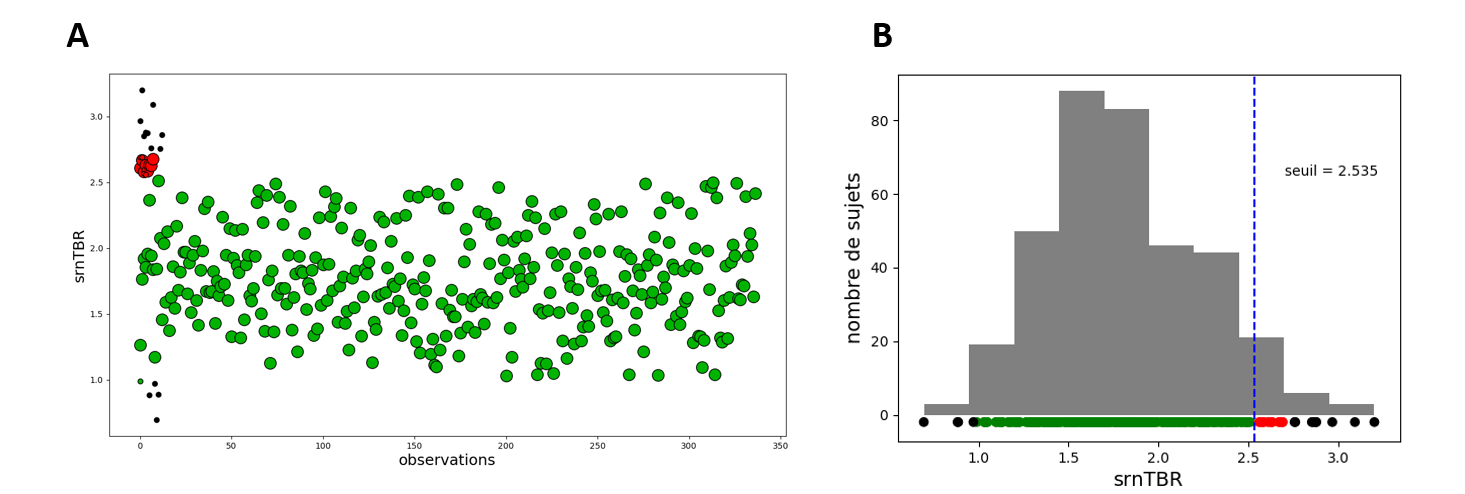
\includegraphics[width=1.0\linewidth]{figures/chapter-4/tbr-dbscan-clustering-plot} 
  \caption[Partitionnement obtenu par \gls{dbscan}.]{Partitionnement obtenu par \gls{dbscan}. Deux groupes sont identifiés (en vert et rouge) et 13 points sont considérés comme du bruit (en noir).
	En \textbf{A} le partitionnement est représenté par un nuage de points et en \textbf{B} sous forme d'histogramme. Le seuil \gls{srntbr} est représenté par 
	la droite verticale en pointillés bleus en \textbf{B}. En \textbf{A} les observations ont été ordonnées de façon à ce que toutes celles du groupe des \gls{tbr} élevés 
	soient regroupées.}
  \label{Figure:tbr_dbscan_clustering_plot}
\end{figure}

Le groupe de \gls{srntbr} élevés (en rouge) contient peu d'observations et est très dense : ces valeurs varient peu d'un sujet à l'autre.


\subsection{Seuils identifiés}
Etant donné que les méthodes utilisées ici concluent toutes qu'un partitionnement des \gls{srntbr} en deux groupes est pertinent, il est possible de s'intéresser
au seuil qui permet de discriminer les données. Ce seuil est calculé pour toutes les méthodes sur les valeurs de \gls{srntbr} : pour convertir le seuil sur 
les valeurs de \gls {tbr}, il suffit de calculer le carré du seuil \gls{srntbr}. Les valeurs de seuil présentées par la suite correspondent au seuil
sur les données \gls{tbr}.

Les seuils obtenus sont : 
\begin{description}
\item[pour le \gls{bgmm} : ] le seuil identifié est de 3.7, il est représenté par un point bleu à la Figure~\ref{Figure:tbr_bgmm},
\item[pour le \gls{gmm} : ] le seuil identifié est de 3.8, valeur très proche de celle du seuil déterminé par le \gls{bgmm},
\item[pour la méthode de Ward : ] le seuil identifié lorsque le nombre de partitions est fixé à 2 est de 4.032, représenté
par une ligne verticale en pointillés bleus à la Figure~\ref{Figure:tbr_ward_histograms},
\item[pour le \gls{dbscan} : ] le seuil identifié est de 6.426, schématisé à la Figure~\ref{Figure:tbr_dbscan_clustering_plot} par une ligne
verticale en pointillés bleus. 
\end{description}

Le courbe \gls{roc} calculée sur le \gls{bgmm} à deux composantes ajustant les \gls{srntbr} est tracée à la Figure~\ref{Figure:tbr_roc} et 
présente une \gls{auc} de 0.872. Sur cette courbe sont ajoutés les seuils obtenus par les autres méthodes et l'\gls{acc} à laquelle ils conduisent. 
La valeur des seuils affichée correspond au seuil sur les valeurs \gls{tbr}. 

\begin{figure}[h!]
  \centering
	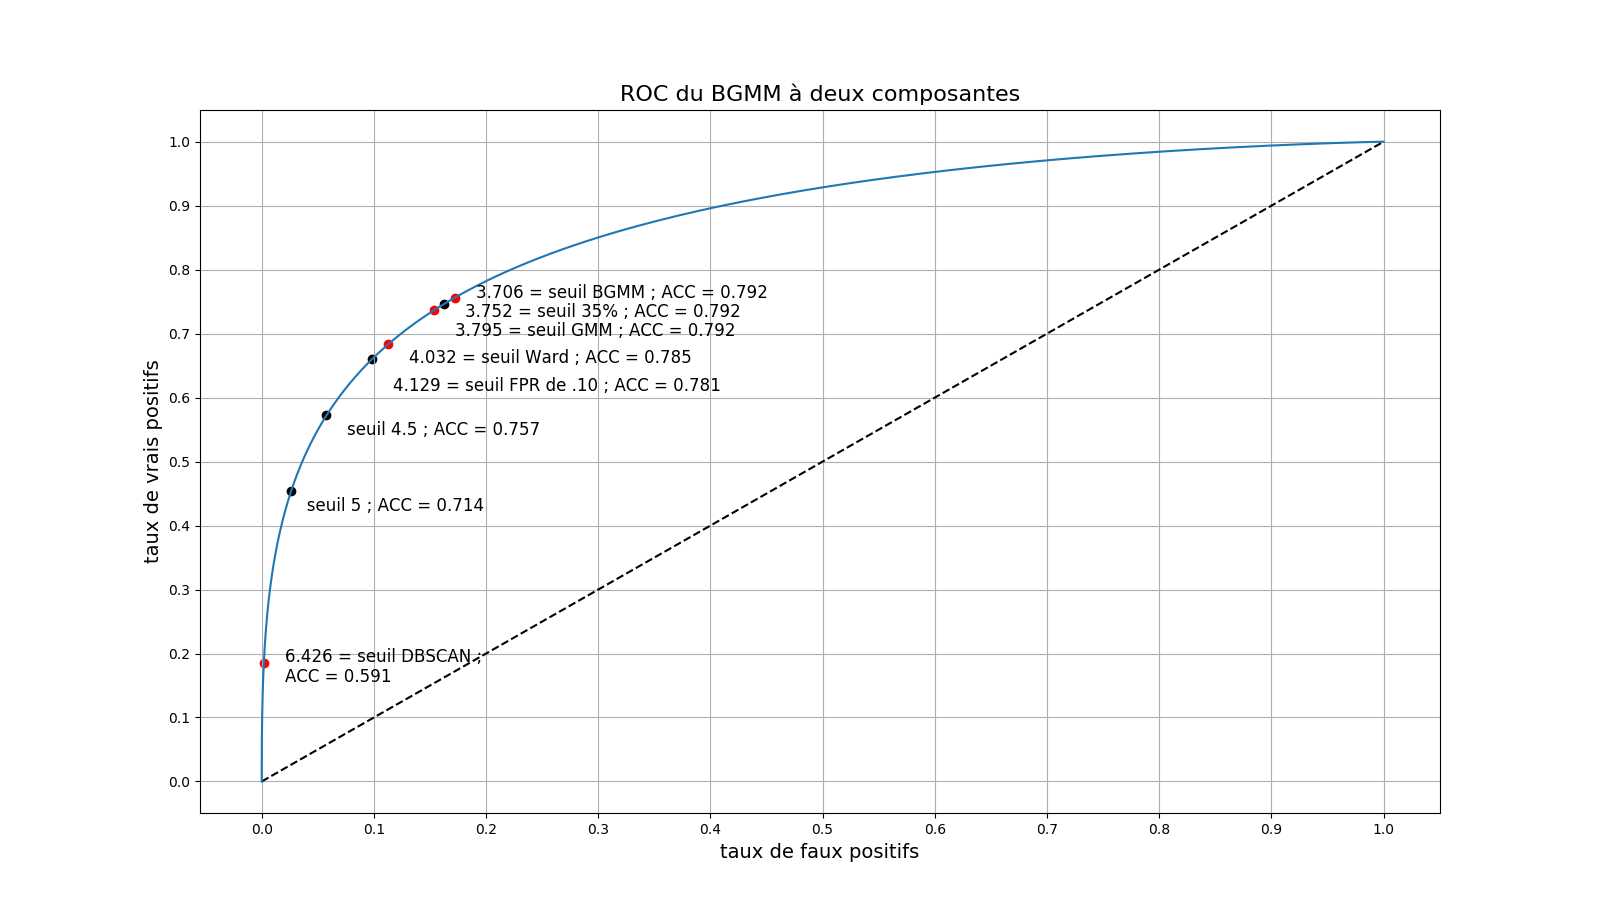
\includegraphics[width=1.0\linewidth]{figures/chapter-4/tbr-roc} 
  \caption[Courbe \gls{roc} obtenue avec le \gls{bgmm} à deux composantes.]{Courbe \gls{roc} obtenue avec le \gls{bgmm} à deux composantes (en bleu). Les seuils \gls{tbr} obtenus avec les méthodes implémentées ici sont représentés 
	par un point rouge sur la courbe ; les seuils issus de la littérature sont représentés par un point noir. Pour chaque seuil la valeur de justesse (\gls{acc}) 
	est donnée.}
  \label{Figure:tbr_roc}
\end{figure}

Les seuils obtenus par les \gls{bgmm} et \gls{gmm} à deux modes et le seuil séparant 35\% de la population étudiée sont ceux conduisant à la plus grande \gls{acc} :
79.2 \%. Les deux seuils menant à des \gls{acc} bien plus faibles sont celui égal à 5 et celui trouvé par \gls{dbscan} avec respectivement une \gls{acc} de 71.4\%
et de 59.1\%. Toutefois, cette faible \gls{acc} est en partie compensée par un plus faible taux de faux positifs.

La Table~\ref{Table:tbr_thresholds_number_of_subjects} résume le nombre de sujets attribués au groupe \gls{tbr} élevés en discriminant les données 
avec les seuils présentés sur la courbe \gls{roc} à la Figure~\ref{Figure:tbr_roc}. La taille de ce groupe est assez stable, sauf pour le seuil identifié 
par \gls{dbscan} qui mène à un groupe comprenant seulement 5\% de la population étudiée.
\begin{table}[h!]
  \centering
  \caption[Poucentage de sujets considérés comme présentant un \gls{tbr} élevé pour chaque seuil \gls{tbr} étudié.]{Poucentage 
	de sujets considérés comme présentant un \gls{tbr} élevé pour chaque seuil \gls{tbr} étudié.}
  \fontsize{9}{11}\selectfont
\begin{tabular}{ ccc }
\toprule
Seuil \gls{tbr} utilisé & Valeur du seuil \gls{tbr} & \shortstack{Pourcentage d'observations \\ (sujets) au-dessus du seuil} \\
\midrule
\gls{bgmm} & 3.706 & 36\% \\
35\% & 3.752 & 35\% \\
\gls{gmm} & 3.795 & 33\%\\
Ward & 4.032 & 29\% \\
\gls{fpr} à 10\% & 4.129 & 28\% \\
4.5 & 4.5 & 24\% \\
5 & 5 & 19\% \\
\gls{dbscan} & 6.426 & 5.79\%\\
\bottomrule
\end{tabular}
  \label{Table:tbr_thresholds_number_of_subjects}
\end{table}


\section{Discussion}

Trois méthodes de partitionnement différentes ont été utilisées afin de déterminer si un groupe d'enfants avec un \gls{tbr} élevé existe et, auquel cas, 
le seuil à partir duquel le \gls{tbr} est considéré comme élevé est calculé. Ces résultats sont discutés ici et les limites de cette analyse sont 
explorées.

\subsection{Pré-traitement des données électroencéphalographiques}

Les 363 sujets \gls{tdah} inclus dans cette étude proviennent de différentes bases de données, leurs signaux \gls{eegi} ont donc dû être homogénéisés 
en suivant les étapes décrites en \ref{pré-traitement TBR}. Lors du traitement des signaux issus des bases de données du \gls{cmi}, des canaux ont 
été rejetés et interpolés : il aurait été intéressant de rapporter le nombre de ces canaux ainsi que d'évaluer la qualité de l'interpolation, notamment 
en comparant les spectres en fréquence des signaux gardés et de ceux qui ont été rejetés. 

\subsection{Groupes et seuils identifiés}

\subsubsection{Groupes d'enfants \gls{tdah}}

Le partitionnement par \gls{bgmm} montre que le modèle à deux composantes ajuste la distribution des \gls{srntbr} significativement mieux que le modèle
à une composante ($p\text{-value} = 0.005$). En ce qui concerne la comparaison entre le modèle à 2 composantes et celui à 3 composantes, même si ce dernier présente 
une \textit{log likelihood} un peu plus élevée (-204.790 contre -204.955), il n'y a pas de différence statistiquement significative entre ces deux modèles ($p\text{-value}
= 0.850$). Ainsi, en accord avec le rasoir d'Occam, le modèle le plus simple qui ajuste le mieux la donnée est retenu. Il est important de souligner
qu'ajouter des composantes au modèle va dans la plupart des cas augmenter la \textit{log likelihood}, c'est pourquoi, on s'intéresse à 
la significativité de cette augmentation pour éviter l'\textit{overfitting}. Le modèle \gls{bgmm} à deux composantes décrit donc le mieux la distribution
des valeurs de \gls{tbr}, ce qui indique qu'il existerait deux groupes distincts d'enfants \gls{tdah}, dont un présentant un \gls{tbr} élevé.

Cette conclusion obtenue avec le partitionnement par \gls{bgmm} est confirmée par les résultats du \gls{gmm} qui, par ailleurs, valident le choix de 
l'\textit{a priori} du \gls{bgmm}. 

Il est important de rappeler qu'ici il a été choisi d'estimer la distribution des données par des Gaussiennes suite à la vérification que la distribution des 
\gls{srntbr} est bien normale.

L'\textit{agglomerative clustering} basé sur la distance de Ward montre que l'ensemble des données peut être réparti 
en deux ou trois groupes. Lors du partitionnement en deux groupes, un groupe correspondant aux \gls{tbr} élevés et comprenant 29\% de la donnée
est identifié. Ce groupe est toujours identifié lorsque le partitionnement se fait en trois groupes : le nouveau groupe est formé dans la sous-population
des \gls{tbr} plus faibles. 

La méthode de Ward a déjà été utilisée lors de recherches 
précédentes sur l'identification de sous-groupes chez les enfants \gls{tdah} basée sur l'\gls{eeg} \citep{Clarke2011}. Dans cette étude le partitionnement
se basait sur les puissances totales et relatives dans les bandes de fréquence delta (1.5 - 3.5 Hz), thêta (3.5 - 7.5 Hz), alpha (7.5 - 12.5 Hz) et bêta 
(12.5 - 25 Hz) isolées dans les zones frontales, temporales et centrales et aussi sur l'âge des sujets. Quatre groupes ont été ientifiés : 
\begin{itemize}
\item \emph{Premier groupe :} activité bêta élevée,
\item \emph{Deuxième groupe :} activité thêta élevée avec peu d'alpha et bêta,
\item \emph{Troisième groupe :} activité des ondes lentes élevées et faible activité des ondes rapides,
\item \emph{Quatrième groupe :} activité alpha élevée,
\end{itemize}

Ainsi, un groupe d'enfants \gls{tdah} au \gls{tbr} élevé a également été identifié par \citet{Clarke2011}.

L'algorithme \gls{dbscan} conduit également à deux groupes, dont l'un correspond aux \gls{tbr} élevés avec un \textit{silhouette score} de 0.388 
qui permet d'être assez confiant dans le partitionnement retourné. Parmi les 13 points attribués à 
aucune classe, 9 correspondent à des sujets ayant un \gls{tbr} élevé. La possibilité qu'a cet algorithme de considérer certains points comme bruités, conduit à
une classe de \gls{tbr} élevés très dense. 

Toutefois, il faut garder à l'esprit que le paramètre $\epsilon$ du \gls{dbscan} a été déterminé visuellement : cette valeur peut donc facilement varier et conduire à
un nombre différent de partitions identifiées. 

En conclusion, ces deux dernières méthodes semblent confirmer les résultats du \gls{bgmm} quant à l'existence d'un groupe de \gls{tbr} élevés, ce qui permet 
d'apporter de nouvelles preuves quant à l'hétérogénéité du \gls{tdah} déjà évoquée dans la littérature \citep{Arns2008, Arns2012, Barry2003, Clarke2011, 
Liechti2013, Loo2013, Loo2018}.

\subsubsection{Seuils de partitionnements}

L'hétérogénéité des patients souffrant de \gls{tdah} implique des réponses thérapeutiques différentes. Une meilleure identification des sous-groupes de patients souffrant de 
\gls{tdah} pourrait permettre de personnaliser l'approche thérapeutique et donc d'optimiser son efficacité pour chaque patient. L'existence de deux groupes distincts au sein de la 
population \gls{tdah} basée sur la valeur du \gls{tbr} étaye l'idée que le traitement par \gls{nfb} devrait être différent pour ces groupes. En effet, il semblerait
plus approprié que le protocole de diminution du \gls{tbr} ne soit proposé qu'aux enfants du groupe \gls{tbr} élevés et que les autres enfants entrainent un autre
neuromarqueur, comme par exemple le \gls{smr}. Ce modèle à deux protocoles a été notamment suggéré par \citet{Kerson2013} et \citet{Arns2012} et a été évalué lors 
d'un récent essai clinique (NCT02778360, Mensia Technologies, France, ClinicalTrials.gov, \citep{Bioulac2019}).

L'essai clinique de Mensia Technologies a fixé un seuil de \gls{tbr} à 4.5 qui permet d'assigner les sujets soit au groupe devant augmenter leur \gls{smr}, soit 
au groupe devant diminuer leur \gls{tbr}. La courbe \gls{roc} représentée à la Figure~\ref{Figure:tbr_roc}, montre que choisir un seuil \gls{tbr} égal à 4.5 conduit
à une \gls{acc} de 75.7\% et à un \gls{fpr} qui est environ deux fois plus faible que celui obtenu avec le seuil déterminé par le \gls{bgmm}. Toutefois, 
le \gls{tpr} est plus faible avec le seuil \gls{tbr} à 4.5. En supposant que le but du seuil est de maximiser l'\gls{acc}, le seuil \gls{bgmm} serait le 
plus adéquat, avec une \gls{acc} de 79.2\%.

Le seuil calculé à partir du \gls{bgmm} à deux composantes conduit à un groupe d'enfants au \gls{tbr} élevé représentant 36\% de la population étudiée. 
Ce pourcentage est en accord avec les précédentes études qui concluent qu'entre 25 et 40\% des patients \gls{tdah} présentent un \gls{tbr} élevé \citep{Arns2012}. 
De plus,\citet{Clarke2011} trouve que 35\% des patients \gls{tdah} ont un \gls{tbr} élevé. 
Les seuils identifiés par les méthodes utilisées ici permettent de former un groupe d'enfants \gls{tdah} présentant un \gls{tbr} élevé comprenant entre
25 et 40\% de la population totale, sauf dans le cas du \gls{dbscan} qui identifie un groupe
de \gls{tbr} élevés comprenant seulement 5.79\% de la population. Ce faible pourcentage ainsi que la basse \gls{acc} obtenue laisse à penser
que la valeur de ce seuil ne sépare pas de manière fiable les deux groupes. Le seuil identifié par la méthode de Ward dans le cas de deux groupes
est proche de celui trouvé par le \gls{bgmm} à deux composantes (4 contre 3.7), ce qui prouve une nouvelle fois qu'il existe un groupe d'enfants \gls{tdah}
présentant un \gls{tbr} élevé.

Au moment de choisir un seuil pour attribuer le protocole d'entrainement par \gls{nfb}, le seuil le plus précis n'est pas nécessairement le meilleur choix.
En effet, optimiser l'\gls{acc} revient à utilser le seuil du \gls{bgmm} de 3.7. Cependant, si on suppose que le protocole de diminution du \gls{tbr} est plus 
efficace pour les patients dans le groupe des \gls{tbr} élevés tandis que le protocole alternatif est efficace de la même façon pour tous les patients, il 
serait préférable de minimiser le \gls{fpr} plutôt que de maximiser l'\gls{acc}. Si on fixe raisonnablement un seuil menant à 10\% de \gls{fpr}, un seuil de 4.1
est obtenu, résultant en un \gls{tpr} de 67\% et une \gls{acc} de 78\%. Cette valeur de seuil a été choisie car un faible \gls{fpr} est intéressant pour traiter 
les patients qui appartiennent au sous-groupe \gls{tbr} élevé avec un protocole adapté à leur profil \gls{eegi}, comme la diminution du \gls{tbr}.

Au vu de ces réultats, nous recommandons l'utilisation d'un seuil \gls{tbr} de 4.1 pour attribuer
les protocoles d'entrainement du fait de son bon équilibre entre un faible \gls{fpr} et une \gls{acc} et un \gls{tpr} élevés. 

Toutefois, il faut garder à l'esprit que ces \gls{acc} sont théoriques car elles n'ont pas été obtenues à l'aide d'un \textit{gold standard} mais grâce au \gls{bgmm}
à deux composantes dont on suppose que les groupes ont été correctement estimés. 

\subsection{Variabilité du calcul des Theta-Beta ratios} 

Comme souligné en \ref{tbr_computation}, la façon dont est calculé le \gls{tbr} est très variable dans la littérature. En effet diverses définitions du \gls{tbr} existent :
il peut être un ratio des puissances ($\mu$V$^2$), des densités de puissance ($\mu$V$^2$/Hz), des tensions ($\mu$V) ou des densités de tensions ($\mu$V/Hz) 
\citep{Liechti2013}. 

De plus, pour une même définition, différents algorithmes de calcul peuvent être utilisés ce qui mène à des écarts entre les valeurs de \gls{tbr}. En 
effet, \citet{Kerson2019} ont montré que la façon dont est gérée la fuite spectrale (\textit{spectral leakage} en anglais), c'est à dire le fait que la puissance
sur une fréquence donnée se disperse sur d'autres fréquences, est une des principales raisons de l'écart entre deux valeurs de \gls{tbr}. 

Par ailleurs, la définition des bandes de fréquence pour calculer le \gls{tbr} peut aussi varier : par exemple, le \gls{tbr} peut être obtenu à partir
de bandes de fréquence standards ou personnalisées, notamment grâce à l'\gls{iapf} du sujet. Ainsi, pour pouvoir comparer les valeurs de \gls{tbr} provenant de différentes
études, une définition homogène doit être mise en place. De récentes études suggèrent de se baser sur des bandes de fréquence 
qui seraient propres à chaque individu \citep{Zhang2017, Saad2018} pour s'affranchir de l'influence de l'âge. A travers cette analyse, nous recommandons de définir le \gls{tbr} de la façon suivante : 
le ratio entre la puissance dans la bande theta et la puissance dans la bande beta, avec une bande theta correspondant à [\gls{iapf} - 5Hz ; \gls{iapf} - 1Hz]
et une bande beta à [\gls{iapf} + 3Hz ; \gls{iapf} + 12Hz]. Ces intervalles ont été définis par la comité scientfique de NEWROFEED. 

Il est important de souligner que les résultats de cette étude sont comparés à ceux où les \gls{tbr} sont calculés à partir de bandes de fréquence standards
les yeux fermés \citep{Zhang2017, Clarke2011}. Ces valeurs de \gls{tbr} sont donc différentes, mais nous supposons que les tendances dans la distribution et le
partitionnement obtenues ici doivent y être observées. Le choix d'effectuer nos analyses sur des données \gls{eegi} enregistrées les yeux ouverts est dû à l'indisponibilté
d'autant de données obtenues les yeux fermés.

\subsection{Analyse des facteurs de confusion}

Les conclusions de cette analyse de la distribution des \gls{tbr} au sein de la population d'enfants \gls{tdah} doivent prendre en compte ces limitations.
En effet, deux points ont été approfondis ici pour juger de leur impact sur les résultats.

\subsubsection{Correction des artefacts oculaires}

La première source d'erreur possible de cette analyse est que les artefacts oculaires n'ont pas été corrigés sur les signaux \gls{eegi}. Ces artefacts de basse fréquence
peuvent affecter les calculs de puissance et donc par ricochet les valeurs de \gls{tbr}. Les distributions des valeurs de \gls{tbr} sans et avec 
la correction d'artefacts oculaires basée sur la séparation aveugle de sources (\textit{blind source separation} en anglais) \citep{Barthelemy2017} 
ont été tracées à la Figure~\ref{Figure:tbr_eye_artifact_correction} où aucune grande différence entre les deux distributions n'est observée. Par conséquent, la correction des artefacts 
oculaires ne semble pas influencer les valeurs de \gls{tbr} calculées. 

Une des hypothèses justifiant ce 
résultat serait que les artefacts oculaires présents dans la bande bêta seraient compensés par ceux de la bande thêta. En effet, le \gls{tbr} est un ratio dont les bandes de
fréquence sont extraites sur les mêmes électrodes. Par ailleurs, même s'il a été montré que les clignements d'yeux affectent davantage la bande thêta que bêta \citep{Barthelemy2017},
la bande thêta ne s'étend que sur 4Hz, contrairement à la bande bêta qui est plus longue (9Hz), ainsi l'hypothèse de la compensation paraît cohérente.


\begin{figure}[h!]
  \centering
	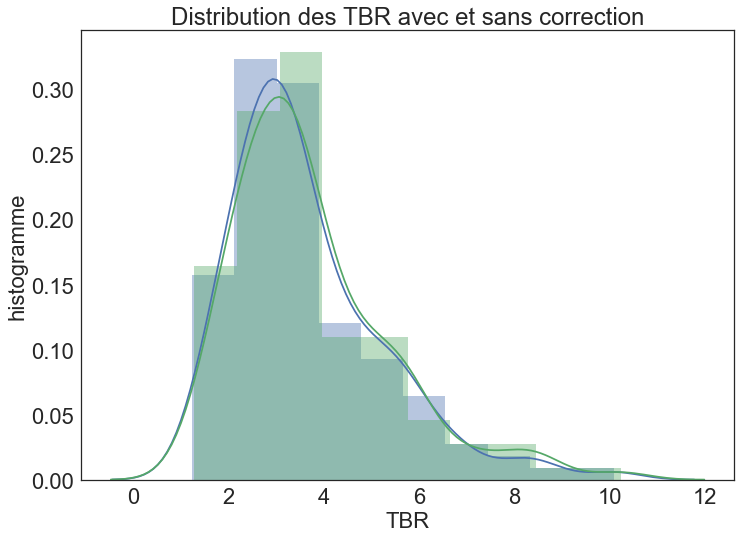
\includegraphics[width=0.7\linewidth]{figures/chapter-4/tbr-eye-artifact-correction} 
  \caption[Comparaison des distributions normalisées de \gls{tbr} calculés après correction des artefacts 
	oculaires et sans correction.]{Comparaison des distributions normalisées de \gls{tbr} calculés après correction des artefacts oculaires (en bleu) et sans correction (en vert).}
  \label{Figure:tbr_eye_artifact_correction}
\end{figure}

\subsubsection{Influence de l'âge}

Une autre source d'inexactitude pourrait être l'âge des sujets inclus dans l'analyse. En effet, la littérature a montré que les valeurs de \gls{tbr} varient
avec l'âge des enfants \citep{Liechti2013, Snyder2015, Perone2018}. De plus, le U-test de Mann-Whitney a été appliqué à nos données \gls{tbr} et a montré
qu'il existe une différence significative entre l'âge des enfants du groupe de \gls{tbr} plus faibles et celui des enfants au \gls{tbr} élevé définis avec 
le seuil de 3.7 du \gls{bgmm} à deux composantes
($p\text{-value} = 2.30e-15$\text{,} $U = 22 104$, avec les âges médians $\pm$ l'ecart absolu médian de chaque groupe : 8.0$\pm$1.57 et 10.1$\pm$2.43). Par ailleurs, lorsqu'on trace
la distribution des âges dans chaque groupe, représentée à la Figure~\ref{Figure:tbr_age_distribution}, on observe que le groupe de \gls{tbr} plus faibles (en vert) comporte 
davantage de sujets âges que le groupe de \gls{tbr} élevé (en rouge). 

\begin{figure}[h!]
  \centering
	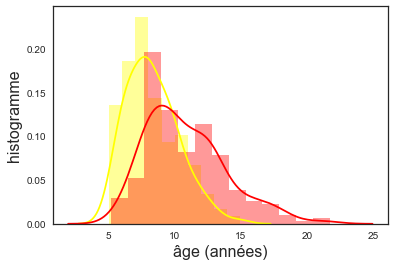
\includegraphics[width=0.7\linewidth]{figures/chapter-4/tbr-age-distribution} 
  \caption[Comparaison des distributions normalisées des âges dans les groupes de \gls{tbr} identifiés par le \gls{bgmm} à deux composantes.]{Comparaison des distributions 
	normalisées des âges dans les groupes de \gls{tbr} identifiés par le \gls{bgmm} à deux composantes. La distribution
	en rouge correspond aux sujets inclus dans le groupe des valeurs de \gls{tbr} élevées et celle en vert au groupe dont les valeurs sont normales.}
  \label{Figure:tbr_age_distribution}
\end{figure}

Ainsi, afin de prendre en compte cette relation, le \gls{bgmm} a été relancé une seconde fois sur un intervalle d'âges plus restreint : seuls les enfants
entre 7 et 13 ans sont inclus, ce qui correspond à un total de 560 sujets \gls{tdah} et de 53 sujets sains. les résultats obtenus sur cette nouvelle population 
conduisent à la même conclusion que sur l'intégralité de la population : deux groupes sont significativement identifiés ($p$-value entre le \gls{bgmm} à 1 et 2 
composantes $= 2e-4$) et un seuil \gls{tbr} de 3.84 est trouvé. 

Etant donné que les variations de \gls{tbr} sont censées augmenter avec l'âge, il serait intéressant d'effectuer cette analyse sur une sous-population de jeunes (5 
à 6 ans) et plus grands (18 à 21 ans) sujets. Cependant, faute d'un nombre suffisant de sujets dans ces extrêmes, cette étude ne peut pas être menée. Les prochaines
études sur le \gls{tbr} devront corriger les valeurs de \gls{tbr} de façon à ce qu'elles ne soient pas affectées par l'âge des patients.

\subsubsection{Autres facteurs de confusion}

Deux facteurs de confusion ont pu être explorés, cependant il en existe d'autres qu'il n'est ici pas possible d'étudier faute de disponibilité des données.
En particulier, même si tous les enfants inclus dans cette étude sont diagnostiqués \gls{tdah}, ils ne présentent sans doute pas tous la même sévérité de symptômes : il serait
intéressant d'étudier si les groupes \gls{tbr} identifiés ici diffèrent significativement au niveau clinique. 

En outre, il a été montré que la présence de comorbidités, comme les troubles du comportement et la dépression, a une influence sur la valeur du \gls{tbr} \citep{Loo2013}. 
\citet{Barry2003erp} ont également souligné que les enfants souffrant des symptômes d'inattention et d'hyperactivité ont tendance à avoir un \gls{tbr} plus élevé que ceux présentant seulement des
troubles d'attention .  

Par ailleurs, il a été observé que les enfants nés en fin d'année sont plus souvent diagnostiqués \gls{tdah} \citep{Layton2018} : en effet ces derniers 
étant parfois plus jeunes de près d'un an, ils peuvent présenter un comportement différent de leurs pairs qui peut amener à un diagnostic du \gls{tdah}. Evaluer si 
les deux groupes d'enfants mis en évidence ici se distinguent par le mois de naissance serait intéressant.

Enfin, un autre facteur qu'il aurait été intéressant d'étudier est l'exposition aux écrans. De nombreuses études se sont penchées sur le lien 
entre troubles de l'attention et temps passé devant les écrans durant l'enfance : alors que les premiers résultats montrent effectivement un lien 
entre les deux \citep{Swing2010, Christakis2004}, de nouvelles études sont venues nuancer cette conclusion \citep{Schmidt2008, Lillard2011, Zimmerman2007, Kostyrka2017}.
En effet, le type de programme regardé par l'enfant aurait une infuence importante : les programmes éducatifs n'auraient pas d'effet négatif sur 
la capacité d'attention.


\section{Conclusion}

Cette étude avait pour but d'explorer l'existence d'un groupe d'enfants souffrant de \gls{tdah} basée sur leur \gls{tbr} extraits de signaux \gls{eegi} enregistrés les yeux 
ouverts. Les résultats montrent qu'il existerait deux groupes : un avec un \gls{tbr} élevé, et l'autre avec des valeurs de \gls{tbr} plus faibles. Bien que les 
distributions de ces deux groupes se superposent, le seuil de séparation le plus précis est de 3.7. Toutefois, le seuil qui équilibre le mieux
le \gls{tpr} et le \gls{fpr} est celui de 4.1, il est donc recommandé pour assigner les protocoles de \gls{nfb}. Par ailleurs, ce travail propose
une recommandation sur la façon de calculer le \gls{tbr}. 

La confirmation de l'existence de deux groupes distincts est importante pour l'utilisation du \gls{nfb} dans le traitement du \gls{tdah}. En effet, cela indique 
qu'un traitement par \gls{nfb} proposant deux protocoles en fonction du \gls{tbr} serait pertinent et pourrait être plus efficace que le même protocole 
de \gls{nfb} appliqué à tout le monde. Toutefois, cette étude n'avait pour but de démontrer ni l'efficacité de la personnalisation du \gls{nfb} ni celle du protocole de diminution de \gls{tbr} chez les 
enfants \gls{tdah} présentant un \gls{tbr} élevé. Alors que certaines études notent une amélioration des symptômes à l'issue d'un protocole \gls{tbr}, 
d'autres obtiennent des résultats plus négatifs. Une possible explication de ce manque d'efficacité reporté dans ces études serait que contrôler 
un ratio de fréquence se révèle plus complexe que de moduler la puissance dans une simple bande de fréquence \citep{Rogala2016}. 
